\documentclass[a4paper,twoside,12pt]{book}
%% === nezbytné balíčky:
\usepackage[T1]{fontenc}    % kódování písma
%\usepackage[IL2]{fontenc}  % kódování písma

\usepackage[utf8]{inputenc}     % vstupní znaková sada tohoto dokumentu: UTF-8
%\usepackage[cp1250]{inputenc}  % vstupní znaková sada tohoto dokumentu: Windows 1250
%\usepackage[latin2]{inputenc}  % vstupní znaková sada tohoto dokumentu: ISO Latin 2

\usepackage[czech]{babel} % česky psaná práce, typografická pravidla. Překládejte pomocí "latex.exe" nebo "pdflatex.exe"
%\usepackage{czech} % česky psaná práce. Překládejte pomocí "pdfCSlatex.exe" ("cslatex.exe" asi bude mít problém s balíkem geometry)
	
\usepackage[a4paper, hmarginratio=3:2]{geometry} % využití A4 stránky a nastavení okrajů (u vazby bude širší)

\usepackage{pdfpages} % pokud nemáte formulář "Zadání bak./dipl. práce" naskenovaný jako PDF, tak ZAKOMENTUJTE
\usepackage[hidelinks]{hyperref} % v PDF budou klikací odkazy ("hidelinks" je nebude rámovat)

%% === balíčky, které se mohou hodit:
%\usepackage{encxvlna} % postará se o spojky a předložky, které dle českých pravidel nesmí být na konci řádku. Dokumentace: http://texdoc.net/texmf-dist/doc/generic/encxvlna/encxvlna.pdf (chová se správně k "vnitřku" listings?)

\usepackage{graphicx} % balíček pro vkládání rastrových grafických souborů (PNG apod.)
%\usepackage{epsfig} % balíčky pro vkládání grafických souborů typu EPSs
\usepackage{float} % rozšířené možnosti umístění obrázků

\graphicspath{{./Kapitoly/1/Obrazky/} {./Kapitoly/2/Obrazky/} {./Kapitoly/3/Obrazky/} {./Kapitoly/PrilohaA/Obrazky/} {./Kapitoly/PrilohaB/Obrazky/}}

%\usepackage{caption} % pro popisky obrázků, tabulek atd.

\usepackage{tabularx} % rozšířené možnosti tabulek
%\usepackage{tabu} % jiný balík pro rozšířené možnosti tabulek

\usepackage{listings}  % balíček vhodný pro ukázky zdrojového kódu v~textu práce/příloh. Nutno nastavit! http://ftp.cvut.cz/tex-archive/macros/latex/contrib/listings/listings.pdf
\usepackage{amsmath} % balíček pro pokročilou matematickou sazbu
\usepackage{amsfonts}
\usepackage{color} % pro možnost barevného textu
%\usepackage{fancybox} % umožňuje pokročilé rámečkování

%\usepackage{index} % nutno použít v případě tvorby rejstříku balíčkem makeindex
%\newindex{default}{idx}{ind}{Rejstřík} % zavádí rejstřík v případě použití balíku index


\frenchspacing % za větou bude mezislovní mezera (v anglických textech je mezera za větou delší)
\widowpenalty=1000 % "síla" zákazu vdov (= jeden řádek ze začátku odstavce na konci stránky)
\clubpenalty=1000 % "síla" zákazu sirotků (= jeden řádek/slovo z konce odstavce samostatně na začátku stránky)
\brokenpenalty=1000 % "síla" zákazu zlomu stránky za řádkem, který má na konci rozdělené slovo

\topmargin=-15mm      % horní okraj trochu menší
\textwidth=150mm      % šířka textu na stránce
\textheight=240mm     % "výška" textu na stránce


\pagenumbering{arabic} % číslování stránek arabskými číslicemi
\pagestyle{plain}      % stránky číslované dole uprostřed

\parindent=0pt % odsazení 1. řádku odstavce
\parskip=7pt   % mezera mezi odstavci

\newcommand{\ti}{\textit} % zkrácený příkaz pro kurzívu
\newcommand{\tb}{\textbf} % zkrácený příkaz pro tučné písmo


%% --- zde jsou zavedeny některé "konstanty" - některé musíte změnit! --- %%
\newcommand{\cvut}{České vysoké učení technické v~Praze}
\newcommand{\fjfi}{Fakulta jaderná a fyzikálně inženýrská}
\newcommand{\ksi}{Katedra softwarového inženýrství}
\newcommand{\program}{Aplikace informatiky v přírodních vědách} % změňte, pokud máte jiný stud. program
\newcommand{\obor}{--} % změňte, pokud máte jiný obor

\newcommand{\druh}{Diplomová práce} % nebo "Diplomová práce"
\newcommand{\woman}{} % pokud jste ŽENA, ZMĚŇTE na: ...{\woman}{a} (je to do Prohlášení)

\newcommand{\logoCVUT}{
\includegraphics{./Zadani+Grafika/symbol_cvut_konturova_verze_cb.pdf}} % logo ČVUT -- podle grafického manuálu ČVUT platného od prosince 2016. Pokud nevyhovuje PDF-verze, tak použijte jinou variantu loga: https://www.cvut.cz/logo-a-graficky-manual -> "Symbol a logo ČVUT v Praze"). Pokud chcete logo úplně vynechat, zadejte místo "\includegraphics{...}" text "\vspace{35mm}"

% přesně podle formuláře "Zadání bak./dipl. práce" VYPLŇTE:
\newcommand{\nazevcz}{Algoritmy strojového učení pro adaptaci autonomních agentů v 3D akční hře}    % český název práce (přesně podle zadání!)
\newcommand{\nazeven}{Machine Learning Algorithms for Adapting Autonomous Agents in a 3D Action Game}          % anglický název práce (přesně podle zadání!)
\newcommand{\autor}{Bc. Martin Jochec}   % vyplňte své jméno a příjmení (s akademickým titulem, máte-li jej)
\newcommand{\vedouci}{Ing. Josef Nový, Ph.D.} % vyplňte jméno a příjmení vedoucího práce, včetně titulů, např.: Doc. Ing. Ivo Malý, Ph.D.
\newcommand{\pracovisteVed}{\ksi, \fjfi, \cvut} % ZMĚŇTE, pokud vedoucí Vaší práce není z KSI
\newcommand{\konzultant}{} % POKUD MÁTE určeného konzultanta, NAPIŠTE jeho jméno a příjmení
\newcommand{\pracovisteKonz}{} % POKUD MÁTE konzultanta, NAPIŠTE jeho pracoviště

% podle skutečnosti VYPLŇTE:
\newcommand{\rok}{2026}  % rok odevzdání práce (jen rok odevzdání, nikoli celý akademický rok!)
\newcommand{\kde}{Praze} % studenti z Děčína ZMĚNÍ na: "Děčíně" (doplní se k "prohlášení")

\newcommand{\klicova}{hry, umělá inteligence, adaptace, autonomní agent, strojové učení}   % zde NAPIŠTE česky max. 5 klíčových slov
\newcommand{\keyword}{games, artificial intelligence, adaptation, autonomous agent, machine learning}       % zde NAPIŠTE anglicky max. 5 klíčových slov (přeložte z češtiny)
\newcommand{\abstrCZ}{Tato diplomová práce se zabývá algoritmy strojového učení pro adaptaci autonomního agenta na chování uživatele ve 3D akční hře. Hlavním cílem je vytvořit jednoduchého autonomního agenta, který dokáže přizpůsobit své chování i vybavení protihráči. Práce představuje existující herní agenty, jako jsou AlphaStar, OpenAI Five a Voyager, a popisuje některé algoritmy a techniky používané při jejich vývoji – například Proximal Policy Optimization nebo Self-Play. Dále se zaměřuje na použité technologie, například Unreal Engine či NevarokML, a na samotný návrh, který je s jejich pomocí realizován. Závěrem jsou výsledky experimentu vyhodnoceny.}    % zde NAPIŠTE abstrakt v češtině (cca 7 vět, min. 80 slov)
\newcommand{\abstrEN}{This thesis focuses on machine learning algorithms for adapting an autonomous agent to user behavior in a 3D action game. The main objective is to create a simple autonomous agent capable of adjusting its behavior and equipment in response to the player. The work introduces existing game agents such as AlphaStar, OpenAI Five, and Voyager, and describes some of the algorithms and techniques used in their development – for example, Proximal Policy Optimization and Self-Play. It then focuses on the technologies used, such as Unreal Engine and NevarokML, and the design that is implemented using them. Finally, the results of the experiment are evaluated.} % zde NAPIŠTE abstrakt v angličtině

\newcommand{\podekovani}{Děkuji Ing. Josefu Novému, Ph.D., za vedení mé diplomové práce a za případnou pomoc při její tvorbě.} % NAPIŠTE poděkování, např. svému vedoucímu:
% Děkuji Ing. Eleonoře Krtečkové, Ph.D. za vedení mé bakalářské práce a za podnětné návrhy, které ji obohatily.
% NEBO:
% Děkuji vedoucímu práce doc. Pafnutijovi Snědldítětikaši, Ph.D. za neocenitelné rady a pomoc při tvorbě bakalářské práce.


\begin{document}
%%%%%%%%%%%% TITULNÍ STRANA -- na následujících cca 30 řádků NESAHEJTE!!!  Generuje se AUTOMATICKY %%%%%%%%%%%%
\thispagestyle{empty}

\begin{center}
	{\LARGE
		\cvut\par
		\fjfi
	}
    \vspace{10mm}

    \begin{tabular}{c}
		\tb{\ksi} \\[3pt]
		\tb{Program: \program}\\   
		\tb{Specializace: \obor}\\
    \end{tabular}

   \vspace{10mm} \logoCVUT \vspace{15mm} 

   {\huge \tb{\nazevcz}\par}
   \vspace{5mm}   
   {\huge \tb{\nazeven}\par}
   
   \vspace{15mm}
   {\Large \MakeUppercase{\druh}}

   \vfill
   {\large
    \begin{tabular}{ll}
    Vypracoval: & \autor\\
    Vedoucí práce: & \vedouci\\
    Rok: & \rok
    \end{tabular}
   }
\end{center}

\clearpage{\pagestyle{empty}\cleardoublepage} % prázdná stránka za tou "titulní", bez čísla

%%%%%%%%%%%% ZADÁNÍ PRÁCE %%%%%%%%%%%%
% Zadání (podepsané děkanem!) musíte NASKENOVAT. Ideálně jako 2stránkové PDF (soubor "zadani_cele.pdf"). 
% Před svázáním to v jednom výtisku VYMĚNÍTE ZA ORIGINÁLNÍ ZADÁNÍ (podepsané děkanem fakulty)!
\newpage  % SEM NESAHEJTE!
\thispagestyle{empty} % SEM NESAHEJTE!

%% zde podle toho, jak jste zadání naskenovali, VYBERTE variantu A, B nebo C:
%
% --- varianta A: zadání naskenované jako 2stránkové PDF:
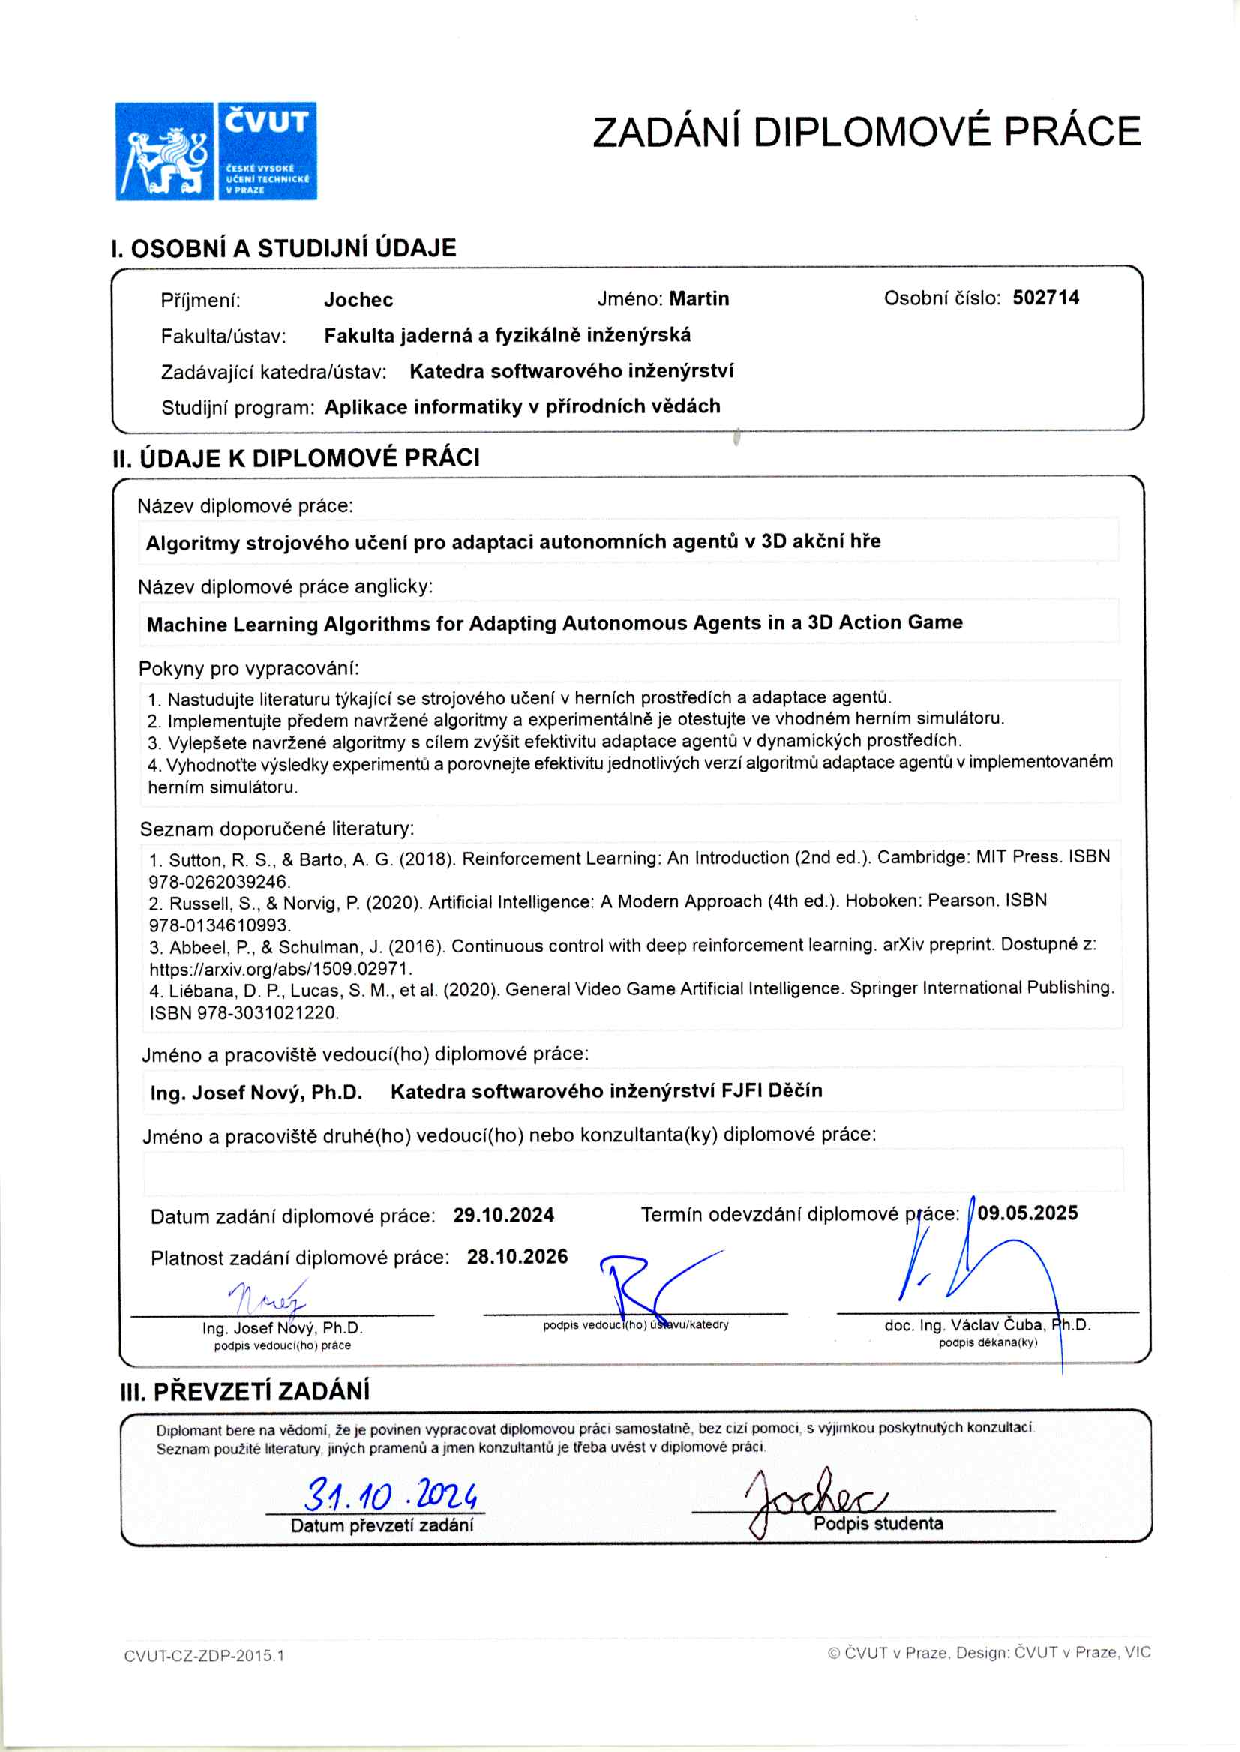
\includepdf[pages={1}]{./Zadani+Grafika/Zadani.pdf} % NAHRAĎTE správným souborem!
%
%% --- varianta B: zadání naskenované jako jednotlivé stránky:
%\includepdf[pages={1}]{zadani1.pdf} % 1. strana zadání v PDF
%\includepdf[pages={1}]{zadani2.pdf} % 2. strana zadání v PDF
%
%% --- varianta C: zadání naskenované jako 2 samostatné obrázky:
%% 1. strana zadání
%\begin{center}
%     \includegraphics[width=1\textwidth]{zadani1.jpg}
%\end{center}
%% 2. strana zadání
%\newpage  % SEM NESAHEJTE!
%\thispagestyle{empty} % SEM NESAHEJTE!
%\begin{center}
%     \includegraphics[width=1\textwidth]{zadani2.jpg}
%\end{center}


%%%%%%%%%%%% Prohlášení  %%%%%%%%%%%%
\newpage % SEM NESAHEJTE!
\thispagestyle{empty}  % SEM NESAHEJTE!


\includepdf[pages={1}]{./Zadani+Grafika/Prohlaseni.pdf} % NAHRAĎTE správným souborem!


%%%%%%%%%%%% Poděkování  %%%%%%%%%%%%
\newpage
\thispagestyle{empty}

~
\vfill % prázdné místo


% -- následující kus kódu (do "%%%%%%%%%%%% ABSTRAKT") můžete odstranit, pokud nechcete psát poděkování:
\tb{Poděkování}

\vspace{1em} % vertikální mezera
\podekovani
\begin{flushright}
\autor
\end{flushright}  % <------- tady končí stránka s poděkováním


%%%%%%%%%%%% ABSTRAKT atp. Je generován AUTOMATICKY podle maker nastavených na začátku souboru) %%%%%%%%%%%% 
\newpage   % SEM NESAHEJTE!
\thispagestyle{empty}   % SEM NESAHEJTE!

% příprava:    (na následujících 8 řádků NESAHEJTE!)
\newbox\odstavecbox
\newlength\vyskaodstavce
\newcommand\odstavec[2]{%
    \setbox\odstavecbox=\hbox{%
         \parbox[t]{#1}{#2\vrule width 0pt depth 4pt}}%
    \global\vyskaodstavce=\dp\odstavecbox
    \box\odstavecbox}
\newcommand{\delka}{120mm} % šířka textů ve 2. sloupci tabulky

% použití přípravy:    % dovnitř "tabular" vůbec NESAHEJTE!
\begin{tabular}{ll}
  {\em Název práce:} & ~ \\
  \multicolumn{2}{l}{\odstavec{\textwidth}{\bf \nazevcz}} \\[1em]
  {\em Autor:} & \autor \\[1em]
  {\em Studijní program:} & \program \\
  {\em Specializace:} & \obor \\
  {\em Druh práce:} & \druh \\[1em]
  {\em Vedoucí práce:} & \odstavec{\delka}{\vedouci\\ \pracovisteVed} \\
  {\em Konzultant:} & -- %\odstavec{\delka}{\konzultant \\ \pracovisteKonz}  % VYMAŽTE text "-- %" v případě, že jste neměli konzultanta
 \\[1em]  
  \multicolumn{2}{l}{\odstavec{\textwidth}{{\em Abstrakt:} ~ \abstrCZ  }} \\[1em]
  {\em Klíčová slova:} & \odstavec{\delka}{\klicova} \\[2em]

  {\em Title:} & ~\\
  \multicolumn{2}{l}{\odstavec{\textwidth}{\bf \nazeven}}\\[1em]
  {\em Author:} & \autor \\[1em]
  \multicolumn{2}{l}{\odstavec{\textwidth}{{\em Abstract:} ~ \abstrEN  }} \\[1em]
  {\em Key words:} & \odstavec{\delka}{\keyword}
\end{tabular}



%%%%%%%%%%%% Obsah práce ... je generován AUTOMATICKY %%%%%%%%%%%%
\newpage  % SEM NESAHEJTE!
\parskip=0pt
\tableofcontents % SEM NESAHEJTE!
\parskip=7pt
\newpage % SEM NESAHEJTE!


%--------------------------------------------------------
%|         Zde začíná SAMOTNÁ PRÁCE (text)              |
%--------------------------------------------------------

\chapter*{Úvod} % SEM NESAHEJTE!
\addcontentsline{toc}{chapter}{Úvod} % SEM NESAHEJTE!

Tato diplomová práce se zabývá algoritmy strojového učení pro adaptaci autonomního agenta na chování uživatele ve 3D akční hře. Hlavním cílem je navrhnout jednoduchého autonomního agenta, který se pomocí strojového učení a~změny vybavení dokáže přizpůsobit protivníkovi a~porazit ho.

První kapitola obsahuje dvě podkapitoly. První se věnuje vybraným technikám a~algoritmům strojového učení, jako jsou Proximal Policy Optimization (PPO), Deep Q-Network (DQN), a~techniky Self-Play a~Population Based Training (PBT). Druhá podkapitola popisuje existující herní agenty, konkrétně AlphaStar, OpenAI Five a~Voyager, včetně přehledu jejich fungování a~způsobu implementace.

Druhá kapitola se zaměřuje na použité technologie a~návrh samotné hry. První podkapitola podrobně popisuje využití Unreal Engine, Visual Studia a~pluginu Nevarok ML, který rozšiřuje Unreal Engine o~funkcionalitu pro trénink a~aplikaci modelů strojového učení. Druhá podkapitola se věnuje návrhu herního prostředí a~autonomního agenta.

Třetí kapitola popisuje implementaci hry a~agenta. První část se zaměřuje na herní logiku, která poskytuje prostředí pro aplikování agenta. Druhá část se věnuje implementaci samotné logiky agenta, pokusům o~vylepšení jeho logiky a~porovnání různých verzí.

Závěr shrnuje úvahy autora a~dosažené výsledky — zda se agent adaptuje podle očekávání, jaký vliv mají jednotlivá vylepšení a~jak si různé verze modelu vedou ve vzájemném porovnání.

\chapter{AI agenti ve hrách a jejich algoritmy a techniky}

\section{Strojové učení a~algoritmy zpětnovazebního učení}

Strojové učení je samostatná oblast umělé inteligence, která se zabývá vývojem metod umožňujících
počítačovým systémům automaticky zlepšovat své chování na základě zkušeností bez nutnosti explicitního
programování všech rozhodovacích pravidel. Takové systémy se učí přímo z~příkladů nebo interakcí
s~prostředím, identifikují vzory a~vytvářejí modely, které generalizují i~na nové situace, jež
nebyly přímo obsaženy v~tréninkových datech.

Takový přístup je zásadní zejména tam, kde ruční definice pravidel nevede k~dobrému výsledku – například
při řízení autonomních agentů v~komplexních, nelineárních a~stochastických prostředích nebo při
adaptivním rozhodování v~dynamických situacích, které nelze přesně popsat jednou sadou pravidel.

Obecně rozlišujeme několik hlavních paradigmat strojového učení, z~nichž každé má své typické úlohy a~metody:

\begin{enumerate}
    \item \textbf{Učení s~učitelem (Supervised Learning)} – modely se učí na označených datech, kde
    jsou vstupy i~správné výstupy známé, a~cílem je minimalizovat rozdíl mezi predikcemi modelu a~
skutečnými výstupy.
    \item \textbf{Učení bez učitele (Unsupervised Learning)} – model hledá strukturu nebo vzory v~
neoznačených datech bez explicitně definovaných výstupů.
    \item \textbf{Částečně řízené učení (Semi-Supervised Learning)} – kombinuje omezené množství
    označených dat s~velkým množstvím neoznačených dat pro efektivnější učení.
    \item \textbf{Zpětnovazební učení (Reinforcement Learning, RL)} – agent se učí sekvenci rozhodnutí
    pomocí interakcí s~prostředím, kdy dostává odměny podle kvality svých akcí \cite{Sutton2018}.
\end{enumerate}

V~této práci se zaměřujeme výhradně na zpětnovazební učení. RL se liší od ostatních paradigmat
především tím, že agent nepracuje pouze s~pevnými daty, ale aktivně ovlivňuje svět kolem sebe,
sleduje výsledky svých rozhodnutí a~učí se na základě toho. Tento způsob učení se formálně modeluje
pomocí \textit{Markovských rozhodovacích procesů (MDP)} – matematického rámce pro rozhodování v~
prostředí s~náhodnými přechody.

MDP je definován jako pětice $(\mathcal{S},\mathcal{A},P,R,\gamma)$, kde:

\begin{itemize}
    \item $\mathcal{S}$ je množina možných stavů prostředí,
    \item $\mathcal{A}$ je množina možných akcí, které může agent vykonat,
    \item $P(s' \mid s,a)$ je přechodová pravděpodobnost, tj. pravděpodobnost, že agent skončí ve stavu
    $s'$ poté, co ve stavu $s$ zvolí akci $a$,
    \item $R(s,a)$ je okamžitá odměna přidělená agentovi za provedení akce $a$ ve stavu $s$,
    \item $\gamma \in [0,1]$ je diskontní faktor, který určuje, jak moc si agent cení budoucích odměn
    vůči těm bezprostředním \cite{Sutton2018}.
\end{itemize}

Agent volí akce podle tzv. \textit{politiky} $\pi(a\mid s)$ – funkce, která pro každý stav $s$ přiřazuje
pravděpodobnost výběru akce $a$. RL algoritmy se snaží nalézt optimální politiku $\pi^*$, která maximalizuje
očekávanou sumu diskontovaných odměn za dlouhé časové horizonty.

\subsection{Proximal Policy Optimization (PPO)}

Proximal Policy Optimization (PPO) je jeden z~nejrozšířenějších algoritmů hlubokého zpětnovazebního učení,
který byl navržen výzkumníky OpenAI jako efektivní a~stabilní alternativa k~dřívějším policy gradient a~trust region
metodám \cite{PPOOpenAI}\cite{Schulman2017}\cite{Jochec2024}. PPO spojuje relativní jednoduchost implementace s~vysokou
stabilitou učení a~efektivním využitím nasbíraných dat.

Na rozdíl od hodnotových metod, jako je Q-learning \cite{Watkins1992}\cite{Sutton2018}, které se snaží
nejprve odhadnout hodnoty stavů či stav-akce a~teprve poté z~nich generovat politiku, PPO přímo optimalizuje
politiku parametrizovanou parametry $\theta$ (např. vahami neuronové sítě). Cílem je nalézt taková
parametry $\theta$, která vedou k~maximalizaci dlouhodobé očekávané odměny.

Klíčovým problémem u~jednodušších policy gradient metod je to, že jednotlivé aktualizace mohou
způsobit příliš velké změny v~politice, což může destabilizovat proces učení. Metody jako TRPO
(Trust Region Policy Optimization) řeší tento problém zavedením explicitních omezení na velikost
kroku při aktualizaci politiky, ale tyto přístupy jsou výpočetně náročné a~komplikované na implementaci
\cite{Schulman2015}. PPO tento problém řeší pomocí tzv. \textit{clipped surrogate objective}, která
udržuje aktualizace politiky v~kontrolovaném intervalu bez složitých optimalizačních podproblémů.

\newpage

Nejprve se zavádí poměr pravděpodobností mezi novou a~starou politikou:

\begin{equation}
r_t(\theta) = \frac{\pi_\theta(a_t\mid s_t)}{\pi_{\theta_{\text{old}}}(a_t\mid s_t)},
\end{equation}

kde $\pi_\theta$ je nová politika, $\pi_{\theta_{\text{old}}}$ je politika před aktualizací, $s_t$
je aktuální stav a $a_t$ akce zvolená ve stavu $s_t$. Tento poměr udává, jak moc se změnila
pravděpodobnost výběru konkrétní akce mezi starou a~novou politikou.

Poté se definuje \textit{oříznutý surrogate loss}:

\begin{equation}\label{eq:ppo_clip_latex}
L^{\text{CLIP}}(\theta) = \hat{\mathbb{E}}_t\left[\min\left(
r_t(\theta)\,\hat{A}_t,\ 
\operatorname{clip}\big(r_t(\theta),1-\epsilon,1+\epsilon\big)\,\hat{A}_t
\right)\right],
\end{equation}

kde:
\begin{itemize}
    \item $\hat{A}_t$ je odhad tzv. \textit{advantage funkce}, která udává, jak moc je akce $a_t$
    ve stavu $s_t$ lepší oproti průměrnému chování,
    \item $\epsilon$ je hyperparametr určující rozsah, ve kterém změna politiky není penalizována,
    \item $\operatorname{clip}$ ořízne hodnotu $r_t(\theta)$ do intervalu $[1-\epsilon, 1+\epsilon]$,
    čímž se minimalizují příliš velké změny politiky \cite{Schulman2017}.
\end{itemize}

Výraz \eqref{eq:ppo_clip_latex} říká, že pokud je změna politiky menší než povolené pásmo dané
$\epsilon$, ponechá se původní hodnota. Pokud je změna větší, bere se hodnota oříznutá na hranici
přijatelného rozsahu. Tento postup zabraňuje vykročení politiky do oblastí, kde by mohla být
nová politika nestabilní nebo výrazně horší než ta původní.

\newpage

Obrázek~\ref{obrPPO} vizualizuje architekturu PPO a~jeho interakci s~prostředím:

\begin{figure}[H]
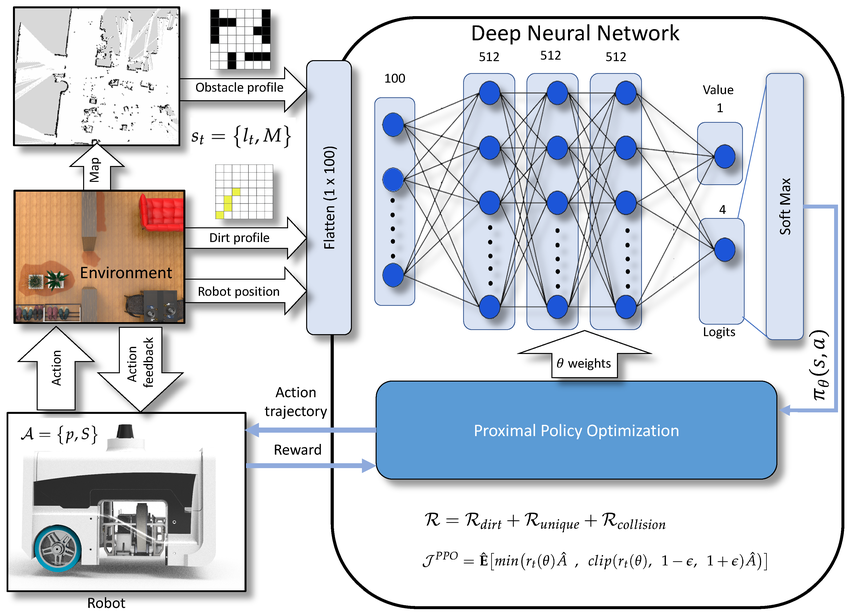
\includegraphics[scale=4]{1-4.png} 
\centering
\caption{Vizualizace architektury algoritmu PPO. Agent je ovlivňován prostředím, zatímco dvě neuronové sítě — actor a~critic — slouží k~výběru akcí a~odhadu hodnoty stavu. Politika se aktualizuje pomocí oříznutého objektivu (clipped objective) a~výhody se počítají pomocí metody Generalized Advantage Estimation (GAE).\cite{PPO2021}}
\label{obrPPO} 
\end{figure}

PPO lze dále rozšířit o~dodatečné složky, které stabilizují učení a~podporují exploraci prostředí:

\begin{equation}
L^{\text{PPO}}(\theta) =
\hat{\mathbb{E}}_t\left[L^{\text{CLIP}}_t(\theta)-c_1\,L^{\text{VF}}_t(\theta)+c_2\,\mathcal{S}(\pi_\theta,s_t)\right],
\end{equation}

kde $L^{\text{VF}}$ je ztráta hodnotové funkce, $\mathcal{S}(\pi_\theta,s_t)$ entropie politiky ve
stavu $s_t$ a $c_1,c_2$ jsou váhové koeficienty určující jejich vliv na celkový loss \cite{Schulman2017}.

\newpage

\subsection{Deep Q-Network}

Algoritmus Deep Q-Network (DQN)\cite{Sutton2018}\cite{Mnih2013}\cite{Jochec2024}\cite{Mnih2015} představuje metodu zpětnovazebního učení, která kombinuje klasický Q-learning\cite{QLearning} s~hlubokými neuronovými sítěmi pro aproximaci akčně-hodnotové funkce \(Q(s,a;\theta)\). Tato funkce udává očekávanou kumulovanou diskontovanou odměnu, kterou agent získá, pokud ve stavu \(s\) provede akci \(a\) a~poté pokračuje optimálním chováním.

Teoretickým základem DQN je Bellmanova optimální rovnice:

\begin{equation}
Q^*(s_t,a_t)=\mathbb{E}\Big[r_{t+1}+\gamma\,\max_{a'}Q^*(s_{t+1},a')\;\Big|\;s_t,a_t\Big],
\end{equation}

kde \(s_t\) je aktuální stav, \(a_t\) zvolená akce, \(r_{t+1}\) okamžitá odměna, \(s_{t+1}\) následující stav a \(\gamma\in[0,1]\) diskontní faktor, který určuje relativní váhu budoucích odměn oproti bezprostředním.

V~klasickém Q-learningu se toto řeší pomocí aktualizačního pravidla:

\begin{equation}
Q(s_t,a_t)\leftarrow Q(s_t,a_t)+\alpha\Big(r_{t+1}+\gamma\,\max_{a'}Q(s_{t+1},a')-Q(s_t,a_t)\Big),
\end{equation}

kde \(\alpha\) je rychlost učení. Pro prostory se stovkami či tisíci stavů by taková tabulka byla nepraktická nebo nemožná. DQN proto využívá neuronovou síť parametrizovanou \(\theta\), která na vstup přijímá reprezentaci stavu \(s\) a~na výstup generuje \textbf{vektor Q-hodnot pro všechny akce}:

\begin{equation}
Q(s,a;\theta)\approx Q^*(s,a).
\end{equation}

Trénink DQN probíhá minimalizací \textbf{časového rozdílu (TD error)} mezi odhadovanou Q-hodnotou a~cílovou hodnotou odvozenou z~Bellmanovy rovnice. Kódování těchto odhadů a~stabilizace učení používá dvě hlavní techniky:

\begin{itemize}
    \item \textit{Přehrávací paměť} (\(\mathcal{D}\)) – ukládá přechody \((s_t,a_t,r_{t+1},s_{t+1})\) a~umožňuje náhodné vzorkování mini-batchů. Tím se přerušuje autokorelace mezi po sobě následujícími vzorky a~zvyšuje se rozmanitost tréninkových dat.
    \item \textit{Cílová síť} – označovaná \(Q(s,a;\theta^-)\), což je periodicky aktualizovaná kopie online sítě. Cílová síť poskytuje stabilní referenční hodnoty během učení.
\end{itemize}

\newpage

Pro výpočet cílové hodnoty a~ztrátové funkce DQN se používají následující výrazy.

Nejprve definujeme cílovou hodnotu \(y_t\):

\begin{equation}
y_t = r_{t+1} + \gamma\,\max_{a'}Q(s_{t+1},a';\theta^-).
\end{equation}

Tento výraz vyjadřuje tzv. \textit{temporal difference target}. Skládá se ze dvou částí:
\begin{itemize}
    \item \textit{Okamžitá odměna} \(r_{t+1}\): okamžitý zisk, který agent získá provedením akce \(a_t\) ve stavu \(s_t\).
    \item \textit{Odhad budoucích odměn} \(\gamma\,\max_{a'}Q(s_{t+1},a';\theta^-)\): diskontovaná hodnota nejlepší možné akce v~následujícím stavu \(s_{t+1}\), podle cílové sítě s~parametry \(\theta^-\). Tento člen reprezentuje odhad kumulativní budoucí odměny.
\end{itemize}

Hyperparametr \(\gamma\) je diskontní faktor, který určuje relativní váhu budoucích odměn vůči bezprostřední odměně. V~praxi se hodnoty \(\gamma\) blíží 1~v~úlohách, kde je důležitý dlouhodobý výsledek, a~menší \(\gamma\) se používá tam, kde jsou odměny krátkodobé.

Následuje výpočet ztrátové funkce \(L_t(\theta)\):

\begin{equation}
L_t(\theta)=\mathbb{E}_{(s,a,r,s')\sim\mathcal{D}}\Big[\big(y_t-Q(s_t,a_t;\theta)\big)^2\Big].
\end{equation}

Tato funkce vyjadřuje \textbf{střední kvadratickou chybu (mean squared error)} mezi:
\begin{itemize}
    \item \textit{aktuálním odhadem} hodnoty Q získaným z~online sítě \(Q(s_t,a_t;\theta)\), kterou trénujeme,
    \item \textit{cílovou hodnotou} \(y_t\), která využívá cílovou síť a~okamžitou odměnu.
\end{itemize}

Minimalizací této chyby učíme síť tak, aby její predikce Q-hodnot co nejlépe odpovídaly cílovým Bellmanovým odhadům. Důležité je, že cílové hodnoty se během tréninku *nepřenastavují okamžitě*, ale fixují se na delší interval pomocí zmíněné cílové sítě \(Q(s,a;\theta^-)\). To zásadně pomáhá stabilizovat učení a~zabraňuje oscilacím nebo divergenci při aktualizaci parametrů.

Po definici loss funkce následuje \textbf{aktualizace parametrů} pomocí gradientního sestupu:

\begin{equation}
\theta\leftarrow\theta-\alpha\,\nabla_{\theta}L_t(\theta),
\end{equation}

kde:
\begin{itemize}
    \item \(\alpha\) je rychlost učení (learning rate), která určuje, jak velký krok do směru negativního gradientu uděláme v~každé aktualizaci,
    \item \(\nabla_{\theta}L_t(\theta)\) je gradient loss funkce vůči parametrům sítě \(\theta\). Tento gradient udává, jak změna každého parametru ovlivní chybu.
\end{itemize}

Gradientní sestup směřuje parametry sítě tak, aby se predikovaná Q-hodnota \(Q(s_t,a_t;\theta)\) blížila cílovému odhadu \(y_t\). V~důsledku toho síť postupně zlepšuje své odhady Q-hodnot pro různé stav-akce páry.

Poslední rovnice vyjadřuje \textbf{synchronizaci parametrů cílové sítě} s~hlavní sítí:

\begin{equation}
\theta^-\leftarrow\theta.
\end{equation}

Tento krok se neprovádí při každé aktualizaci, ale periodicky (např. každých \(K\) tréninkových kroků). V~praxi se tím zajistí, že cílová síť zůstane dostatečně „fixní“ po určitou dobu, což zabraňuje tomu, aby se cílové hodnoty měnily příliš rychle a~destabilizovaly tréninkový proces. Bez této separace by totiž síť během učení upravovala své parametry tak, že by se sama učila na neustále se měnící cílové funkci — což má tendenci vést k~oscilacím nebo divergenci.

Stručně řečeno:
\begin{itemize}
    \item \textit{Loss funkce} měří, jak moc se predikce odchyluje od cílové hodnoty na základě Bellmanovy rovnice.
    \item \textit{Gradientní aktualizace} upravuje váhy tak, aby se tato odchylka minimalizovala.
    \item \textit{Target network} odděluje výpočet cílových Q-hodnot od parametrů, které se právě učí, čímž stabilizuje trénink.
\end{itemize}

Tréninkový cyklus DQN tedy typicky probíhá následovně:

\begin{enumerate}
    \item Sledování aktuálního stavu \(s_t\).
    \item Výběr akce \(a_t\) pomocí \(\epsilon\)-greedy politiky.
    \item Provedení akce, získání odměny \(r_{t+1}\) a~nového stavu \(s_{t+1}\).
    \item Uložení přechodu do paměti \(\mathcal{D}\).
    \item Náhodné vzorkování mini-batchů dat z \(\mathcal{D}\).
    \item Výpočet cílové hodnoty \(y_t\) a~minimalizace TD chyby.
    \item Periodická aktualizace parametrů cílové sítě (\(\theta^- \leftarrow \theta\)).
\end{enumerate}

Algoritmus DQN je citlivý na nestabilitu a~divergenci kvůli kombinaci nelineární aproximace neuronovou sítí a~bootstrapovaných aktualizací. Přehrávací paměť redukuje autokorelaci dat a~zvyšuje efektivitu využití zkušeností, zatímco cílová síť poskytuje stabilnější referenční hodnoty. Pokročilé varianty, jako jsou \textit{Double DQN}, \textit{Dueling DQN} nebo \textit{Prioritized Experience Replay}, rozšiřují základní metodu s~cílem zlepšit konvergenci, stabilitu a~efektivitu učení v~komplexních prostředích.

\begin{figure}[ht]
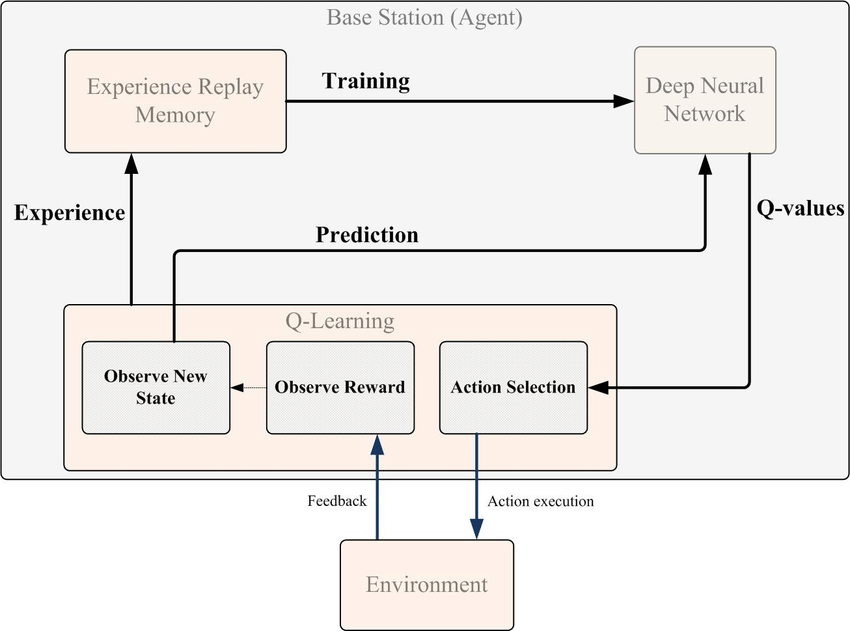
\includegraphics[scale=0.45]{1-7.png} 
\centering
\caption{Příklad architektury Deep Q-Learning\cite{Elsayed2021}}
\label{obrADQL}
\end{figure}

Tyto dva algoritmy byly již zmíněny ve výzkumné práci\cite{Jochec2024}, kde tato diplomová práce na ni navazuje. Teď budou zmíněny dvě trénovací techniky, Self-Play a~Population Based Training.

\newpage

\subsection{Self-Play}

Self-play\cite{Zhang2024} je technika tréninku v~oblasti zpětnovazebního učení, která umožňuje agentům 
zlepšovat své strategie prostřednictvím interakcí s~jinými instancemi sebe sama – typicky s~kopiemi, 
historickými verzemi nebo současnými protivníky založenými na stejné struktuře politiky. Cílem self-play 
je generovat adaptivní tréninková data bez nutnosti externích protivníků či lidského dozoru, čímž se agent 
učí robustní strategii na základě postupného zvyšování úrovně soupeře během tréninku.

Na rozdíl od klasického zpětnovazebního učení, kde agent interaguje se statickým prostředím, self-play funguje 
v~rámci dynamického prostředí, které vytváří další agentní entity, jejichž chování se v~čase vyvíjí a~
reaguje na aktuální strategii. To vede k~učením, která mohou překročit jednoduché optimalizační úlohy a~
dosahovat hlubší strategické adaptace, zejména v~úlohách s~konkurenční povahou.

Základní forma self-play, často označovaná jako \uv{vanilla self-play}, spočívá v~tom, že agent opakovaně 
hraje proti své vlastní nejnovější verzi. Tato metoda funguje efektivně v~prostředích, kde lze strategie 
řadit podle jejich kvality (transitivní hry), protože agent postupně zvyšuje úroveň soupeře sám proti sobě. 
V~prostředích s~ne-transitivní dynamikou může tato jednoduchá forma self-play vést k~cyklickému chování 
a~suboptimálním strategiím.

\newpage

Aby se tyto nevýhody zmírnily, vznikají různé varianty:

\begin{itemize}
    \item \textit{Fiktivní self-play} rozšiřuje trénink tím, že agent hraje proti průměru všech svých 
    předchozích verzí politiky. Tím se zvyšuje robustnost učení a~snižuje riziko zacyklení v~suboptimálních strategiích.
    \item \textit{Prioritizovaná fiktivní self-play} používá vážený výběr soupeřů, kde se preferují ty 
    politiky, proti kterým si agent vede méně dobře – tedy trénuje intenzivněji vůči slabým stránkám vlastní strategie.
    \item \textit{$\delta$-uniform self-play} zavádí hyperparametr $\delta$, který určuje, jaká část 
    historické populace politik se použije jako soupeři. Nižší $\delta$ zahrnuje širší spektrum historických politik, 
    zatímco vyšší $\delta$ dává přednost nedávno generovaným verzím.
\end{itemize}

Self-play se často integruje s~tzv. \textit{population-based} přístupy. Namísto jednoho agenta existuje populace 
politik $\Pi$, která se v~čase rozšiřuje o~nové verze. Každá politika se trénuje vůči soupeřům vybraným z~populace 
na základě určité metastrategie $\Sigma$, často reprezentované interakční maticí nebo distribuční strategií. Tento 
proces vytváří bohatý a~adaptivní prostor pro evoluci strategií a~vzájemnou adaptaci politik.

Základní smyčka self-play s~populací obvykle probíhá následovně:

\begin{enumerate}
    \item Nové politiky jsou inicializovány, často na základě posledních iterací existujících politik.
    \item Každá politika se trénuje proti soupeřům vybraným podle metastrategie $\Sigma$.
    \item Nově natrénované politiky se přidají zpět do populace a~proces se opakuje.
\end{enumerate}

Z~hlediska výpočetní efektivity se rozlišují varianty jako:

\begin{itemize}
    \item \textit{lazy initialization}, kdy se politiky inicializují až v~okamžiku potřeby,
    \item \textit{immediate initialization}, kdy se populace vytvoří celá najednou na začátku.
\end{itemize}

Dále se rozlišuje:

\begin{itemize}
    \item \textit{standardní trénink}, kde se v~každé iteraci trénuje jeden agent,
    \item \textit{průběžný trénink}, kdy se všechny politiky trénují paralelně.
\end{itemize}

Zejména v~kontextu větších populací a~her s~komplexní strategií hraje důležitou roli tzv. PSRO (\textit{Policy-Space Response Oracles}). 
PSRO rozšiřuje klasické self-play tak, že pracuje s~populací politik a~iterativně generuje nejlepší odpovědi na směs politik populace, 
čímž se přibližuje rovnováze typu Nashovy rovnováhy. To je důležité zejména v~nestranově tranzitivních nebo multi-agentních hrách, 
kde jednoduché sebehráčské strategie nemusí konvergovat ke stabilnímu optimu.

\newpage

Self-play nachází využití v~konkurenčních a~multi-agentních prostředích — klasickými příklady jsou hry jako Go, šachy, StarCraft II 
nebo Dota 2 — a~také v~jiných oblastech, například v~některých aplikacích robotiky, kde dynamické protinavádění podporuje robustní 
strategie bez nutnosti lidského tréninkového dozoru.

Obrázek~\ref{obrSPvsPPvsBCP} ilustruje rozdíly mezi přístupy \uv{self-play} (SP), \uv{population-play} (PP) a \uv{behavioral cloning play} (BCP). 
Druhý ze zmíněných přístupů využívá širší populace politik, zatímco BCP je založen na učení z~lidských demonstračních dat, což je odlišné od 
čistě self-play přístupů, které generují data prostřednictvím interakcí agentů mezi sebou.

\begin{figure}[ht]
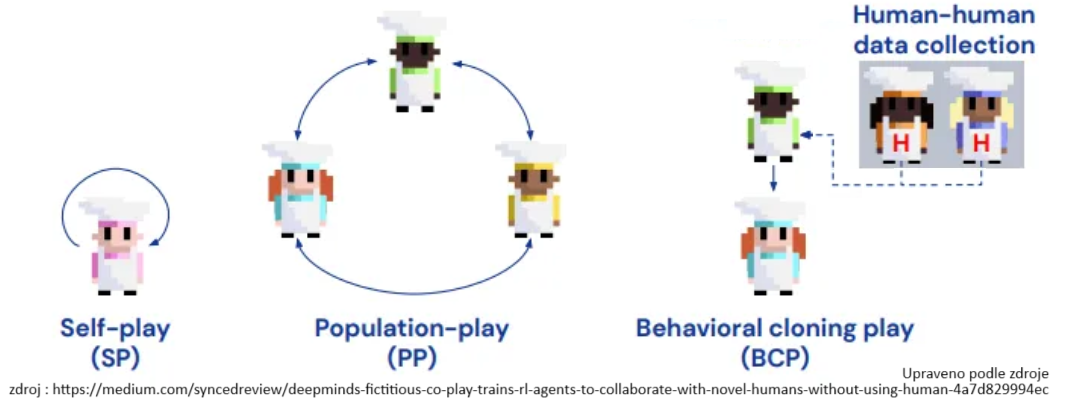
\includegraphics[scale=0.67]{1-5.png} 
\centering
\caption{Srovnání tří přístupů k~tréninku agentů: \uv{self-play} (SP), kde agent hraje sám proti sobě; \uv{population-play} (PP), kde interaguje s~různými agenty v~populaci; a \uv{behavioral cloning play} (BCP), kde se učení zakládá na lidských demonstračních datech. Upraveno podle zdroje\cite{Strouse2021}}
\label{obrSPvsPPvsBCP} 
\end{figure}

\newpage

\subsection{Population Based Training}

Population-Based Training (PBT)\cite{Jaderberg2017} je technika automatického ladění hyperparametrů, která propojuje samotný trénink neuronových sítí s~jejich optimalizací tak, aby se váhy sítě a~její hyperparametry upravovaly současně během jednoho běhu učení. PBT vzniká jako reakce na omezení tradičních metod ladění, jako je grid search nebo Bayesian optimization, které často vyžadují mnoho samostatných tréninků s~fixními konfiguracemi a~mohou být časově i~výpočetně náročné.

V~PBT se nevyhledává pouze jedna nejlepší sada hyperparametrů, ale algoritmus se snaží \textbf{automaticky objevit jejich optimální plán (schedule)} během tréninku samotného modelu — díky tomu se může přizpůsobovat různým fázím učení, kdy různé hodnoty hyperparametrů jsou vhodné v~různých časech tréninku.

Na začátku PBT inicializuje populaci modelů, přičemž každá instance populace má:
\begin{itemize}
    \item vlastní váhy (parametry neuronové sítě),
    \item vlastní konfiguraci hyperparametrů (např. learning rate, entropická penalizace, délka unrollu apod.).
\end{itemize}

Každý model se trénuje paralelně a~nezávisle pomocí běžných optimalizačních metod (např. SGD nebo Adam). V~pravidelných intervalech se populace vyhodnocuje a~provádí tzv. \textit{exploit-and-explore} fáze, které spojují principy evolučních algoritmů s~gradientním učením.

\textit{Exploit} znamená, že modely s~horším výkonem přebírají váhy a/nebo hyperparametry od modelů s~lepším výkonem. Tato operace je analogická selekci v~genetických algoritmech — silnější jedinci „přežijí“ a~jejich parametry se šíří do dalších populací. 
\textit{Explore} znamená, že tyto převzaté hyperparametry jsou \textbf{lehce modifikovány} (např. vynásobením faktorem 1{,}2~nebo 0{,}8), aby populace prozkoumala nové konfigurace. Tím se neustále testují různé kombinace nastavení během tréninku a~umožňuje se adaptivní ladění hyperparametrů bez nutnosti opakovaných běhů tréninku od začátku.

Proces lze shrnout následovně:
\begin{enumerate}
    \item Každý model ve své instanci trénuje standardní metodou s~aktuální konfigurací hyperparametrů.
    \item Po určité době nebo podle metriky se vyhodnocuje výkon každého modelu.
    \item Pokud je model označen jako \uv{ready}, probíhá fáze \uv{exploit} – model si kopíruje váhy a~hyperparametry od výkonnějších modelů v~populaci.
    \item Následuje fáze \uv{explore}, při které se hyperparametry lehce mění (například násobky, malé perturbace nebo náhodné přegenerování).
    \item Trénink pokračuje s~nově nastavenými vahami a~hyperparametry a~celý cyklus se opakuje.
\end{enumerate}

Tento způsob optimalizace kombinuje směry gradientního učení a~evolučního vyhledávání tak, že:
\begin{itemize}
    \item zajišťuje \textbf{adaptivní změnu hyperparametrů během učení},
    \item eliminuje potřebu řešit tréninky s~fixními konfiguracemi opakovaně,
    \item dovoluje paralelní škálování na heterogenních výpočetních systémech bez centrální koordinace.
\end{itemize}

Obrázek~\ref{obrPBT} ilustruje, jak si modely v~rámci populace sdílejí váhy a~mění hyperparametry na základě výkonnosti:

\begin{figure}[ht]
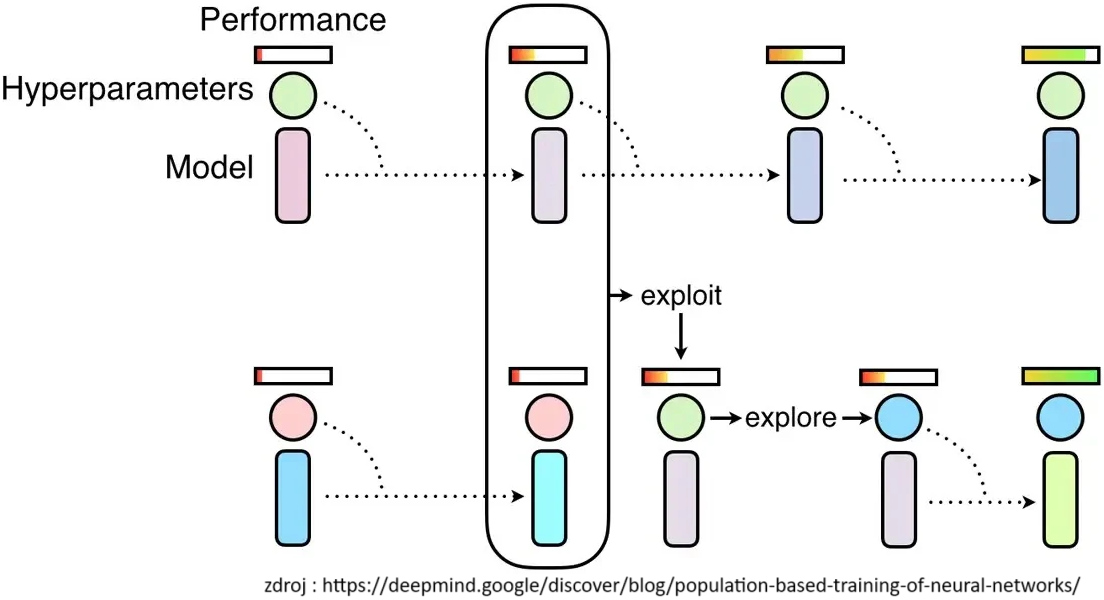
\includegraphics[scale=0.35]{1-6.png} 
\centering
\caption{Population-Based Training neuronových sítí začíná jako náhodné prohledávání, ale v~průběhu tréninku umožňuje jednotlivým modelům využít dílčí výsledky ostatních (fáze \uv{exploit}) a~zároveň zkoušet nové kombinace hyperparametrů (fáze \uv{explore}).\cite{PBT2017} }
\label{obrPBT} 
\end{figure}

Klíčové principy PBT mohou být interpretovány jako hybridní systém:
\begin{itemize}
    \item \textit{výběr modelů} podobný truncation nebo turnajové selekci v~evolučních metodách,
    \item \textit{perturbace hyperparametrů} jako jednoduchý heuristický způsob prozkoumání prostoru hyperparametrů během běhu tréninku,
    \item \textit{asynchronní aktualizace}, která eliminuje nutnost synchronizace všech modelů.
\end{itemize}

Tato technika byla v~původní práci demonstrována na úlohách hlubokého zpětnovazebního učení, kde vedla nejen k~rychlejší konvergenci, ale i~k~vyššímu konečnému výkonu modelů při optimalizaci různých hyperparametrů. PBT také nachází uplatnění v~dalších oblastech, jako je strojové překládání nebo trénink generativních modelů, kde automaticky objevuje sekvence hyperparametrů, které překonávají ručně laděné konfigurace.

Důležitou výhodou PBT je jeho \textbf{online charakter} — ladění hyperparametrů probíhá současně s~tréninkem modelů, což je efektivnější nejen časově, ale i~z~hlediska výpočetních zdrojů, protože se eliminuje potřeba trénovat modely od začátku po každé úpravě hyperparametrů. Tento aspekt výrazně odliší PBT od tradičních metod ladění, které obvykle vyžadují dokončení jednoho tréninkového běhu před dalším experimentem.

Celkově lze PBT vnímat jako techniku, která do procesu učení vnáší adaptivitu, sdílení informací mezi modely a~evoluční principy, což podporuje robustnější a~efektivnější optimalizaci ve srovnání s~pevně danými metodami ladění.

\newpage

\section{AI agenti ve hrách}
\subsection{AlphaStar}

AlphaStar\cite{Vinyalsbr} je agent umělé inteligence (AI) vyvíjený společností DeepMind pro hraní hry StarCraft II\cite{WikiSC}, což je komplexní a~dynamická online strategie v~reálném čase s~částečnou pozorovatelností, rozsáhlým akčním prostorem a~dlouhodobým plánováním. Hra StarCraft II je považována za jeden z~nejnáročnějších testovacích prostorů pro vývoj inteligentních systémů, protože kombinuje strategické a~taktické rozhodování se zpracováním neurčitých informací a~interakcí více agentů.

AlphaStar byla veřejnosti představena v~lednu 2019 a~již v~srpnu téhož roku dosáhla hodnosti \uv{Grandmaster}, což je nejvyšší úroveň na oficiální žebříčkové lize StarCraft II a~znamená, že se agent řadí mezi přibližně 0{,}2\,\% nejlepších lidských hráčů. Tento úspěch představuje významný milník nejen v~oblasti herní AI, ale i~ve vývoji komplexních autonomních systémů, které zvládají vysokodimenzionální rozhodovací úlohy.

StarCraft II jako prostředí klade na agenta řadu výzev, které nejsou přítomné v~jednodušších hrách nebo simulacích: \textbf{časové omezení, skryté informace (fog of war), rozsáhlý akční prostor, dynamické kombinace jednotek a~strategií, a~nutnost plánování na krátkodobé i~dlouhodobé úrovni}. Teprve kombinace moderních technik strojového učení dokázala tyto výzvy překonat.

Vývoj AlphaStar odráží dlouhodobý směr výzkumu DeepMind. Zakladatel Demis Hassabis již v~roce 2011 označil StarCraft za další krok ve výzkumu herní AI po úspěších s~AlphaGo, agentem pro hru Go, který porazil světového šampiona. Po spojení s~Blizzard Entertainment a~zpřístupnění API pro boty v~roce 2017 začal DeepMind zpracovávat historická herní data a~postupně stavět a~trénovat své agentní sítě.

AlphaStar funguje na kombinaci několika technik:
\begin{itemize}
    \item \textit{Učení z~lidských dat}: původní agent byl trénován pomocí imitace strategií z~rozsáhlé databáze anonymních her lidských hráčů, aby se naučil základní struktury herního rozhodování.
    \item \textit{Hluboké zpětnovazební učení (Reinforcement Learning)}: agent dále optimalizoval svou politiku pomocí zpětné vazby ze simulovaných her tak, aby maximalizoval pravděpodobnost vítězství.
    \item \textit{Multi-agentní trénink a~self-play}: agenti hráli proti sobě v~rozsáhlých tréninkových ligách, což umožňovalo objevování a~adaptaci různých strategií bez ručního navrhování pravidel.
    \item \textit{Population-Based Training (PBT)}\cite{Jaderberg2017}: tato technika automaticky ladila hyperparametry během tréninku, čímž zvyšovala efektivitu a~kvalitu učení.
\end{itemize}

AlphaStar je navržen tak, aby zvládal komplexní rozhodovací prostor StarCraft II pomocí hlubokých neuronových sítí, které zpracovávají game-state v~reálném čase a~generují akce, které reflektují kombinaci taktického i~strategického myšlení.

AlphaStar se stal historicky prvním AI systemem, který dosáhl \textbf{hodnosti Grandmaster ve veřejném žebříčku hry StarCraft II} bez umělých omezení algoritmu, čímž překonal většinu lidských hráčů v~rámci oficiálního kompetitivního prostředí. Tento výkon byl dosažen i~přesto, že prostředí kladlo na agenta lidské omezení jako omezené zorné pole kamery a~omezenou rychlost akcí, aby se co nejvíce přiblížilo podmínkám, za kterých hrají lidé.

Model AlphaStar tak představuje \textbf{pokročilou kombinaci imitace, reinforcement learningu, multi-agentního tréninku a~adaptivního ladění}, která umožňuje extrémně komplexní herní rozhodování. Přestože je tento systém navržen primárně pro herní prostředí, principy, které byly při jeho vývoji použity, mají potenciál být aplikovány i~v~jiných oblastech, kde je potřeba řešit nelineární rozhodovací úlohy v~přítomnosti neúplné informace a~dynamických protivníků.

AlphaStar nepředstavuje jedinou strategii, ale udržuje populaci různorodých politik, které odrážejí různé herní styly a~strategie. Tato populace se během tréninku dynamicky rozšiřuje a~přizpůsobuje, čímž se zvyšuje robustnost a~schopnost adaptace agentů v~různorodém prostředí. Tento přístup je úzce spojen s~principy kvalitní diverzity (Quality Diversity, QD), kdy místo jediné optimalizované strategie vzniká více kvalitních, ale odlišných řešení, která jsou vůči sobě navzájem méně zranitelná.

\begin{figure}[H]
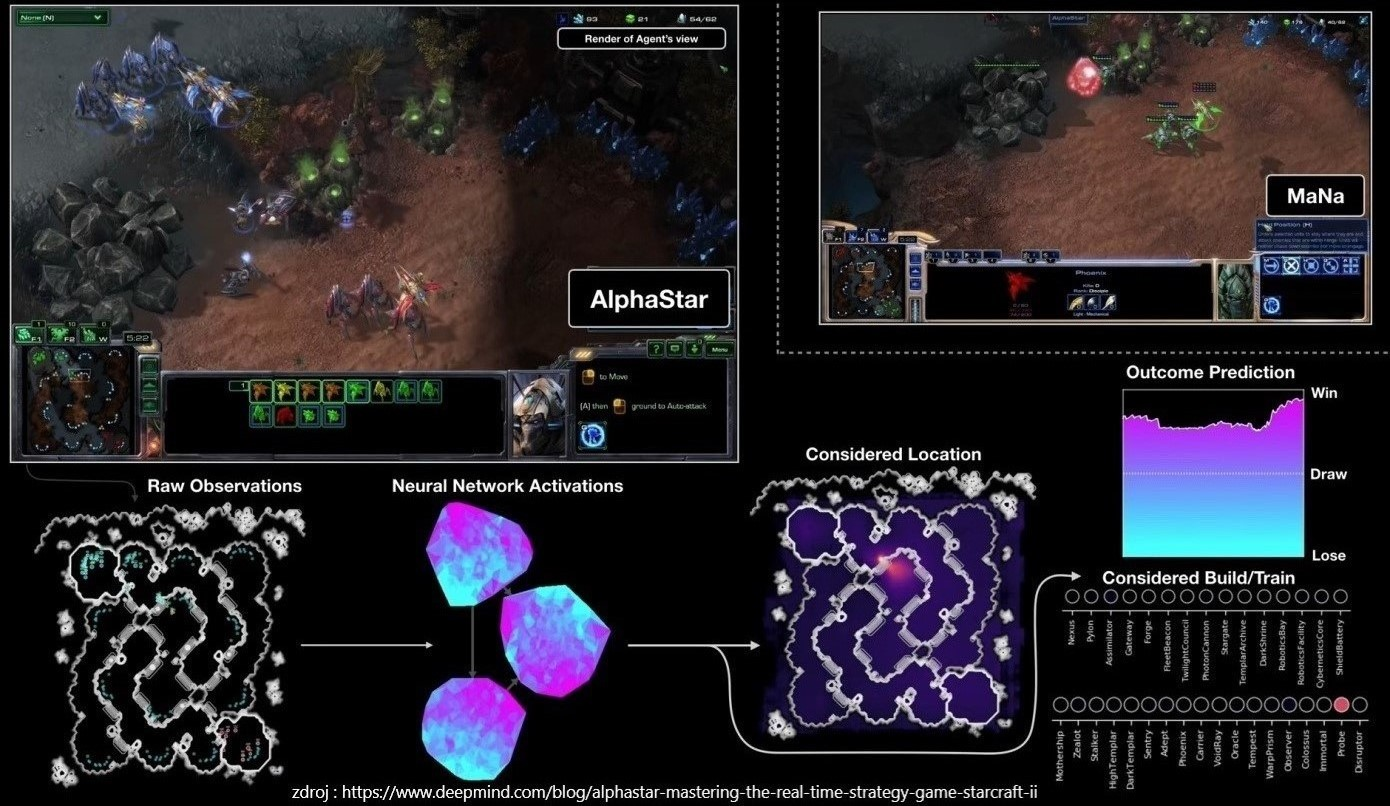
\includegraphics[scale=0.41]{1-1.jpg}
\centering
\caption{Vizualizace rozhodovacího procesu AlphaStaru během zápasu proti hráči. Systém zpracovává syrová pozorování, aktivuje neuronové sítě, vyhodnocuje potenciální akce a~předpovídá výsledky zápasu.\cite{AlphaStar2019}}
\label{obrAlphaStar}
\end{figure}

\newpage

\subsection{OpenAI Five}

OpenAI Five\cite{OpenAIFive} je agent umělé inteligence vyvinutý společností OpenAI, navržený pro hraní týmové videohry Dota 2\cite{Dota2}, ve které proti sobě nastupují dvě pětičlenná družstva. Tato hra představuje jedno z~nejkomplexnějších prostředí pro testování agentů umělé inteligence, protože kombinuje \textbf{dlouhé časové horizonty, částečnou pozorovatelnost a~vysokodimenzionální akční a~stavový prosto¨r}, které výrazně přesahují jednodušší hry jako šachy či Go.

Poprvé se OpenAI Five veřejnosti představuje v~roce 2017 během živé demonstrace na turnaji The International, kde v~duelu jeden na jednoho poráží profesionálního hráče Dendiho — což ukazuje, že agent dokáže získat přehled a~efektivně rozhodovat i~v~takto náročném prostředí. Následující rok systém pokročuje natolik, že zvládá ovládat celý tým pěti agentů a~poráží amatérské i~poloprofesionální lidské soupeře ve formátu 5v5.

Vývoj agentních algoritmů pro OpenAI Five začíná již v~listopadu 2016. OpenAI zvolila Dota 2~jako testovací prostředí mimo jiné kvůli její \textbf{složitosti, nepředvídatelnosti hry, robustnímu API a~vysoké popularitě}, což umožnilo testovat a~měřit výkon agentů v~realistickém konkurenčním scénáři.

OpenAI Five využívá \textbf{framework hlubokého zpětnovazebního učení (deep reinforcement learning)}, přičemž jádrem tréninkové metodiky je algoritmus \uv{Proximal Policy Optimization} (PPO)\cite{PPOOpenAI}\cite{Schulman2017}. PPO je gradientní algoritmus politiky, který kombinuje efektivní využití dat, stabilní učení a~relativně jednoduchou implementaci — což je důležité při škálování učení na rozsáhlé distribuované systémy, jaké OpenAI v~tomto projektu použila. PPO zabraňuje příliš razantním aktualizacím politiky zavedením tzv. oříznutého objektivu (\textit{clipped surrogate objective}), který omezuje změny v~distribučních pravděpodobnostech akcí během gradientních kroků.

Každý agent v~OpenAI Five je reprezentován neuronovou sítí s~jednou vrstvou typu \textbf{LSTM o~4096 jednotkách}, která zpracovává aktuální herní stav získaný přes API Dota 2. Tento stav je zakódován jako vektor zhruba 20 000 číselných hodnot, jež popisují relevantní informace z~herního prostředí, například pozice jednotek, dostupné akce, cooldowny schopností a~další proměnné.

Rozhodování probíhá pomocí několika \textbf{nezávislých akčních hlav}, z~nichž každá odpovídá za jiný aspekt chování agenta — například volbu konkrétní akce, její umístění v~prostoru nebo časování provedení akce. Každý krok agenta je reprezentován osmi číselnými hodnotami (tzv. \uv{action enumeration}), které definují konkrétní volbu v~daném časovém okamžiku.

Trénink OpenAI Five probíhá na rozsáhlé distribuované infrastruktuře nazvané Rapid, která umožňuje masivní paralelní výpočet a~koordinaci tisíců strojů. Díky tomu systém odehrává denně obrovské množství simulovaných her — v~některých fázích tréninku se sbírá ekvivalent více než 180 let herního času na den, což je umožněno paralelním hraním \uv{self-play} na stovkách GPU a~desítkách tisíc CPU jader.

\newpage

OpenAI Five tak neustále trénuje a~optimalizuje své politiky hraním proti sobě samému (\uv{self-play}), přičemž model získává odměny za různé klíčové herní cíle, jako je zabíjení nepřátel, ničení struktur nebo dosahování herních objektivů. Tento proces podporuje postupné zlepšování strategie a~koordinace celého týmu agentů.

Závěrečnou veřejnou prezentací projektu byly exhibiční zápasy v~dubnu 2019, během nichž OpenAI Five poráží tým OG — tehdejší mistry světa z~The International 2018 — ve formátu best-of-three se skóre 2:0~na živém streamu, čímž demonstruje, že jeho výkon překonává i~špičkové lidské profesionály. Během čtyřdenní online akce OpenAI Five dále otestoval své schopnosti v~více než 7~000 zápasech proti veřejným hráčům, z~nichž vyhrál přibližně 99{,}4 \% — což potvrzuje konzistentní a~robustní výkon v~rozsáhlém měřítku.

Díky své robustnosti, efektivitě a~schopnosti fungovat v~distribuovaných systémech je PPO ideálně vhodný pro tuto aplikaci. Umožňuje agentům provádět rozsáhlý paralelní trénink bez přeučení, přičemž jeho kompatibilita se sdílenými politikami i~hodnotovými funkcemi přispívá k~úspěšné koordinaci agentů v~komplexním prostředí Dota 2.

\newpage

\subsection{Voyager}

Voyager\cite{Wangbr} je zástupce tzv. ztělesněných agentů (embodied agents), kteří kombinují výhody velkých jazykových modelů (LLM) s~učením ve složitých, otevřených prostředích. Tento agent funguje autonomně ve hře Minecraft — bez přímého lidského zásahu nebo předem definovaných odměnových funkcí — a~učí se postupně z~vlastních interakcí s~herním světem. Minecraft je pro tento typ agenta ideálním prostředím, protože neobsahuje pevný konec hry, má procedurálně generované světy a~vyžaduje dlouhodobé plánování a~adaptivní rozhodování, což odráží výzvy reálných úloh.

Klíčové vlastnosti Voyagera jsou založeny na třech hlavních mechanismech, které mu umožňují \textbf{otevřené, kontinuální učení bez lidské intervence}:

\begin{enumerate}
    \item \textbf{Automatické kurikulum} – agent si sám generuje sekvenci úkolů na základě aktuálního stavu světa, inventáře a~historie již provedených akcí. Tato posloupnost úkolů maximalizuje exploraci a~postupně vede ke schopnostem potřebným pro složitější dovednosti.
    \item \textbf{Knihovna dovedností} – po úspěšném splnění úkolu agent vytvoří program reprezentující tuto dovednost a~uloží jej do knihovny. Dovednosti jsou indexovány vektorovými embeddingy jejich popisu, což umožňuje jejich pozdější opětovné použití nebo kombinaci s~jinými schopnostmi.
    \item \textbf{Iterativní promptování} – při řešení úkolu agent nejprve navrhne program (např. v~JavaScriptu) pro daný úkol pomocí GPT-4~a~poté jej provede ve hře. Výsledek, včetně chyb a~zpětné vazby z~prostředí, se vrací GPT-4, které program upraví a~iterativně opravuje, dokud není úkol úspěšně dokončen nebo vyhodnocen jako neřešitelný.
\end{enumerate}

Automatické kurikulum nehledá náhodné úkoly, ale generuje je kontextově na základě aktuální situace v~prostředí, což umožňuje efektivní prozkoumávání světa a~dlouhodobé zlepšování agentovy schopnosti učit se.

Dovednosti, které Voyager získá, nejsou izolované akce, ale mohou být hierarchicky složeny. Například dovednost vytvořit železný nástroj může využívat dovednosti jako těžba rudy, výroba pece nebo sběr surovin, přičemž se buduje na znalostech získaných dříve a~minimalizuje hrazené opakování již naučených postupů.

Iterativní promptování je charakteristické tím, že agent nevykonává pouze jednorázové akce, ale \textbf{opakuje cyklus generování a~hodnocení kódu} za použití zpětné vazby z~prostředí. Kód, který selže kvůli chybě, je upraven na základě analýzy chyby a~dalšího promptu, čímž vzniká robustní smyčka učení, která agentovi umožňuje zlepšovat své strategie bez explicitního překalibrování modelu.

Ve srovnávacích experimentech Voyager významně překonává předchozí agentní metody založené na jiných přístupech, jako jsou ReAct či Auto-GPT. Agent získává více unikátních předmětů, pokrývá větší území a~rychleji dosahuje technologických milníků, což ukazuje jeho schopnost adaptovat se a~učit se v~otevřeném prostředí bez ručního ladění cílů.

Celkově lze Voyagera vnímat jako významný krok směrem k~obecné autonomní umělé inteligenci v~otevřených světech, protože demonstruje, že \textbf{agent vybavený LLM a~mechanismy samostatného učení může dlouhodobě akumulovat znalosti, generalizovat získané dovednosti a~přizpůsobovat se novým úlohám bez lidského zásahu}.

\begin{figure}[ht]
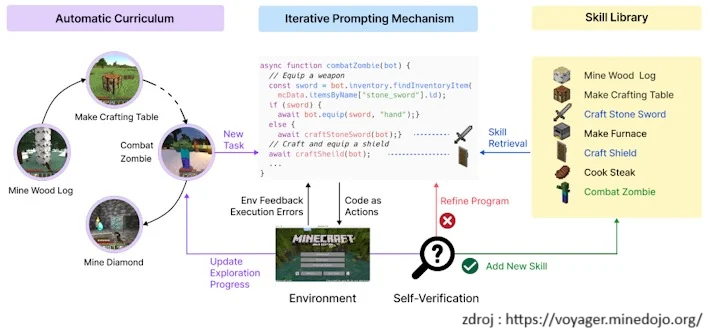
\includegraphics[scale=1]{1-3.png} 
\centering
\caption{Vizualizace hlavních komponent systému Voyager – automatického kurikula, knihovny dovedností a~iterativního promptování.\cite{Voyager2023}}
\label{obrVoyager} 
\end{figure}

\chapter{Použité technologie a návrh hry}

\section{Návrh a implementace prostředí hry}

\section{Návrh a implementace autonomního agenta}

\section{Otestování chování agenta}

\chapter{Implementace hry a agenta, vylepšení jeho algoritmu a porovnání verzí}

\section{Základní logika hry}
\subsection{Hráčská postava}
Po spuštění hry se aktivuje úvodní funkce, která inicializuje několik klíčových podsystémů hráčské postavy. Nejprve se připojí mapa ovládacích vstupů, která umožňuje hráči ovládat pohyb postavy pomocí klávesnice. Následně se k postavě připojí tzv. průhledový displej (HUD), díky kterému se zobrazují herní informace na obrazovce. Součástí této inicializace je také aktivace zaměřovače, který se synchronizuje s HUDem a reaguje na hráčovy vstupy. Další funkce aktivují systémy obnovování – konkrétně regeneraci života, energie a baterie svítilny. Zároveň se zpřístupní sekce HUDu, které tyto parametry zobrazují. Následující část vytváří proměnné potřebné pro propojení postavy v blueprintu s logikou sběru předmětů a obsluhou zbraní. Závěrečná inicializační funkce rozšiřuje HUD o prvek zobrazující typ právě vybavené zbraně.

Pohyb hráčovy kamery je řízen pomocí pohybu myši – horizontálně po ose Z a vertikálně po ose Y. Samotný pohyb postavy po mapě se realizuje zvlášť pro směr vpřed/vzad a pro pohyb do stran. V obou případech se využívají směrové vektory a výsledná hodnota se předává do funkce pro fyzický posun postavy. Systém zároveň detekuje, zda hráč běží či se plíží, aby mohl spustit nebo zastavit příslušné zvukové efekty.

Pro plynulé ozvučení pohybu je využito makro, které opakovaně volá funkci zajišťující přehrávání kroků. Pokud hráč přestal padat (například po skoku), znovu se aktivuje zvuk chůze. Systém zároveň detekuje typ povrchu pod nohama pomocí trasovací linky – podle nalezeného materiálu se přehrává odpovídající zvuk kroků.

\newpage

Běhání je vázáno na dostupnou energii. Pokud hráč neběží a není v podřepu, ale začne se pohybovat a má dostatek energie, hra aktivuje běh. Energie se začne postupně snižovat a změní se rychlost přehrávání zvuku chůze. Jakmile běh ustane, energie se opět pomalu doplňuje a rytmus zvuku se přizpůsobí.

Podobně je řešen i úskok do stran. Pokud má hráč více než 15 bodů energie a není v podřepu, může provést úskok ve směru aktuálně stisknuté pohybové klávesy. Po dokončení úskoku se po krátké pauze začne energie obnovovat.

Při plížení (podřepu) systém kontroluje, zda hráč neběží ani neuskočil a zda má dostatek staminy. Pokud ano, postava se přepne do podřepu, tempo chůze se zpomalí a začne se doplňovat energie. Při návratu do vzpřímené pozice se část energie spotřebuje, ale opět začne regenerace.

Součástí logiky hráčské postavy je také systém pozastavení hry. Po stisknutí příslušného tlačítka se hra přeruší a na obrazovce se zobrazí menu pauzy.

Mechanismus spotřeby a regenerace energie (staminy) je řízen samostatnými funkcemi. Během běhu nebo jiných fyzicky náročných akcí se každým tikem odečítá stanovené množství staminy. Jakmile její hodnota klesne na nulu, postava přestane běžet. Naopak, pokud hráč není aktivně v pohybu, aktivuje se obnova energie, která ji postupně přičítá až do maximální hodnoty.

Postava má také funkce pro správu zdraví. Pokud je hráč zraněn, aktivuje se odečet životů. Následně, pokud postava stále žije, začne pomalá regenerace zdraví. Jakmile hodnota života dosáhne maxima, regenerace se pozastaví. Pokud však zdraví klesne na nulu, postava umírá – ovládání se zablokuje, zvuky se vypnou a zobrazí se obrazovka smrti. Odtud má hráč možnost hru ukončit nebo začít od začátku.

\newpage

\subsection{Zbraňový systém}
Zbraňový systém ve hře je navržen tak, aby simuloval chování střelných zbraní, včetně střelby, přebíjení, sběru munice a interakce s prostředím. Na začátku se vytvoří ukazatel na hráče, což umožňuje přímou interakci mezi zbraní a hráčskou postavou.

Při výstřelu se automaticky odebere jeden náboj ze zásobníku a spustí se dvě animace – jedna vizualizuje samotný výstřel zbraně, druhá animaci hráče při střelbě. Pokud jsou náboje v zásobníku vyčerpány, zbraň začne vydávat charakteristický zvuk prázdného cvaknutí, který hráče upozorní na nutnost přebít.

Přebíjení se spustí pouze tehdy, pokud zásobník není plný. Systém nejprve zjistí, kolik nábojů chybí do plné kapacity zásobníku, a poté doplní chybějící náboje z celkové zásoby. Tento proces je doprovázen přehráním animace přebíjení. Pokud hráč na mapě sebere náboje, ověří se, zda ještě není překročen maximální počet. Pokud ne, náboje se přičtou do celkové zásoby.

K interakci se zbraněmi na mapě slouží dvě specifická tlačítka – tlačítko E pro sběr zbraní ze země a tlačítko B pro jejich odhození. Při sběru zbraně hra detekuje její přítomnost v okolí hráče, načte informace o typu zbraně, aktuálním počtu nábojů v zásobníku a celkové zásobě, a tyto údaje převede do inventáře hráče. Zbraň se následně odstraní ze světa a nahradí ji aktivní zbraň v rukou hráče, která je vizuálně připojena k jeho postavě.

Při odhození zbraně se zbraň v rukou hráče zničí a na místě před hráčem se vytvoří nová zbraň, kterou je možné znovu sebrat.

Logika střelby zohledňuje typ zbraně. Pokud má hráč v ruce automatickou pušku, hra aktivuje opakovanou střelbu, dokud jsou v zásobníku náboje. U brokovnice je implementována funkce náhodného rozptylu projektilů, která simuluje široký zásahový úhel typický pro tento typ zbraně. Brokovnice vystřelí několik střel najednou, každou s mírně odlišnou trajektorií. V případě odstřelovací pušky se spouští klasická střelba s jedním přesným výstřelem.

Střelba je iniciována funkcí, která detekuje rotaci a pozici hráčovy kamery. Ze zbraně je vyslána přímka simulující trajektorii střely, která může ovlivnit nepřátelskou umělou inteligenci. Další paprsek vychází přímo z kamery hráče a končí ve vzdálenosti určené směrem pohledu. Simulace rovněž zohledňuje nepřesnosti způsobené pohybem postavy a náhodný rozptyl u brokovnice.

Po výstřelu dochází k simulaci zpětného rázu, která upraví směr pohledu hráče. Pokud je zasažen nepřítel, aplikuje se poškození. V případě zásahu objektu s fyzikální interakcí se na něj aplikuje síla v opačném směru vůči směru střely.

Každý výstřel také spustí zvukový event, na který mohou nepřátelé reagovat. Zbraň rovněž generuje efekt vyhození prázdné nábojnice – ta po výstřelu vyletí ze zbraně a po určité době automaticky zmizí ze scény.

\newpage

Tlačítko pro přebíjení (R) volá funkci, která spustí výše popsaný proces doplnění zásobníku, čímž je zajištěna plná integrace mezi hráčovými vstupy a systémem správy munice.

Celý zbraňový systém je pečlivě propojen s HUDem, který hráči poskytuje vizuální zpětnou vazbu o typu zbraně, počtu nábojů a stavu zásob.

Agent využívá podobný zbraňový systém, který je však zjednodušený – nevyužívá všechny funkce ani některé modifikátory.

\subsection{Logika řízení herních kol}
Logika řízení herních kol a nepřátelských jednotek ve hře začíná inicializací základních proměnných. Po spuštění úrovně se nastaví ukazatel na hráče, obnoví se hlasitost zvukových efektů podle posledního uloženého nastavení a zavolá se funkce pro zahájení nové herní seance.

V rámci této funkce se resetuje proměnná určující, zda již byli všichni nepřátelé naspawnováni, inkrementuje se čítač aktuálního kola a spustí se časovač, který po uplynutí definované doby aktivuje začátek nového kola.

Zahájení kola zahrnuje nastavení počtu nepřátel, kteří se mají v daném kole objevit. Poté se spustí časovač, který s definovaným zpožděním volá funkci pro výběr náhodného místa spawnování. Na tomto místě se následně vytvoří nová instance nepřítele. Každý nepřítel je implementován jako trenér neuronové sítě, který je součástí tréninkové logiky.

Každý spawnovaný nepřítel je vytvořen na základě pozice a orientace předem definovaných spawnovacích bodů, čímž se zajišťuje variabilita a nepředvídatelnost jednotlivých kol.

Paralelně běží neustále se opakující kontrolní funkce, která monitoruje počet aktivních nepřátel. Jakmile systém detekuje, že byli všichni nepřátelé eliminováni, automaticky aktivuje ukončení aktuálního kola.

Závěrečná funkce každého kola zjišťuje, jakou zbraň měl hráč v ruce a jaké měl nastavené brnění (logika brnění je popsána dále v kapitole), a následně spouští další kolo.

\newpage

\subsection{Systém sbírání předmětů}
Logika sběru herních předmětů je založena na detekci kolize mezi hráčovou postavou a specifickou kolizní sférou umístěnou kolem sbíratelných objektů. Jakmile dojde ke kontaktu těchto dvou komponent, spustí se funkce, která aktivuje možnost interakce a zvednutí daného objektu. Pokud hráč oblast opustí, volání funkce se přeruší a předmět zůstane nedotčen.

Při sběru zbraní kolizní sféra kromě detekce kontaktu uchovává také informace o konkrétní zbrani – například její typ a počet nábojů v zásobníku i celkové zásobě. Po stisknutí příslušné klávesy předá sféra tyto údaje hráčovu blueprintu, čímž dojde k přenosu zbraně do rukou hráče a následnému odstranění objektu ze scény.

Pro sběr nábojů se využívá obdobná logika. Když hráč vstoupí do kolizní oblasti s municí, systém zkontroluje, zda má pro daný typ nábojů (automatická puška, brokovnice, odstřelovací puška) dostatek volné kapacity. Pokud ano, náboje se přidají do odpovídající zásoby. V opačném případě zůstávají na místě a mohou být sebrány později, jakmile bude dostatek prostoru.

\subsection{Herní rozhraní (HUD)}
V hlavním menu má hráč na výběr několik možností. Tlačítko „Play“ spustí samotnou hru. Volba „Controls“ otevře obrazovku, na které jsou vizuálně zobrazeny všechny ovládací klávesy. Možnost „Options“ poskytuje přístup k nastavení hlasitosti, kvality audia a vizuálních parametrů pro optimalizaci výkonu. Změny lze potvrdit tlačítkem „Apply“ nebo zrušit pomocí „Back“. Tlačítko „Quit Game“ slouží k ukončení hry.

Během hraní může hráč kdykoli otevřít pauzovací menu stiskem klávesy P. Toto menu obsahuje stejné volby jako hlavní menu, s výjimkou toho, že tlačítko „Play“ zde slouží k návratu zpět do hry a „Main Menu“ přesměrovává do úvodního menu. Pokud hráč během hry zemře, zobrazí se speciální nabídka se třemi možnostmi: „Restart“ (nové spuštění hry), „Quit to Main Menu“ (návrat do hlavního menu) a „Quit“ (vypnutí hry).

Hlavní herní HUD je komplexní a rozčleněný do několika oblastí. V levém dolním rohu se nacházejí tři informační lišty: horní zobrazuje stav baterie svítilny na zbrani, prostřední udává úroveň zdraví a spodní ukazuje energii postavy. Vedle těchto lišt se zobrazuje číslo aktuálního kola. Pravý dolní roh zobrazuje počet nábojů v zásobníku, počet náhradních nábojů a informace o aktuálně držené zbrani (její název a typ).

Střed obrazovky je vybaven zaměřovačem, jehož velikost se dynamicky mění v závislosti na rychlosti pohybu hráče, což napomáhá přesnějšímu míření. V horní části displeje je umístěn časovač, který odpočítává čas do začátku nového kola. V pravém horním rohu se nachází panel zobrazující změny atributů nepřátel, které vznikají na základě výstupu z neuronové sítě, a nad ním také počítadlo snímkové frekvence (FPS), které slouží ke sledování výkonnosti hry.

\section{Autonomní agent}
\subsection{První verze agenta}
Pro začátek jsem chtěl otestovat, jak probíhá trénování, vytváření modelu a nasazení natrénovaného modulu na simulaci v pluginu NevarokML. Proto jsem se pro první verzi rozhodl vytvořit jednoduchého agenta, který se dokáže pohybovat a postupně si v průběhu tréninku i simulace zlepšovat svou schopnost dosáhnout cíle.

\subsubsection{Trénovací mapa}
Na trénovací mapě se nachází hlavní entita typu NevarokMLTrainer, která slouží k tréninku agenta v rámci pluginu NevarokML. Pod ní funguje 270 podřízených entit typu NevarokMLEnvironment, z nichž každá obsahuje simulovaný herní svět pro konkrétního agenta. V každém prostředí je zároveň přítomna entita \uv{agent}, na níž probíhá samotný trénink nebo simulace.

Dále se v každém prostředí nachází pouze podlaha (bez stěn — v této první verzi nejde o uzavřený prostor), pod kterou je umístěna spouštěcí oblast typu Trigger s názvem AbyssTrigger. Kromě toho je poblíž každého agenta ještě jeden Trigger s názvem GoalTrigger, který slouží jako cíl simulace.

\subsubsection{NevarokMLTrainer}
V NevarokMLTrainer se nejprve nastaví velikost tzv. \uv{Action Space} (akčního prostoru), aby NevarokMLEnvironment věděl, kolik typů akcí může agent provádět — buď jednu po druhé, nebo, pokud je to tak nastavené, i několik akcí během jednoho tiku tréninku či simulace. V první verzi, kdy agent zvládne pouze pohyb, má akční prostor pět akcí, které může provádět sekvenčně.

Dále se připravuje tzv. \uv{Observation Space} (pozorovací prostor), kam agent během hry ukládá určená data sloužící k učení a rozhodování v průběhu tréninku a simulace. Po vytvoření Action Space a Observation Space se aktivuje Blueprint uzel nazvaný PPO, což je algoritmus zvolený pro všechny tři verze tréninku a simulace. Tento uzel definuje klíčové hyperparametry:

\begin{itemize}

\item \uv{Policy = MlpPolicy} — agent používá plně propojenou vícervrstvou perceptronovou síť pro aproximaci politiky i hodnotové funkce.

\item \uv{Learning Rate} — ovlivňuje velikost kroků při aktualizaci vah, nižší hodnota znamená stabilnější, ale pomalejší učení.

\item \uv{N Steps} — počet kroků simulace sbíraných před aktualizací politiky.

\item \uv{Batch Size} — počet přechodů (stav–akce–odměna) zpracovaných v jednom mini‑batchi.

\item \uv{N Epochs} — kolikrát se síť trénuje na nasbíraných datech před jejich zaházením.

\item \uv{Gamma} — diskontní faktor pro budoucí odměny.

\item \uv{GAE Lambda} — vyvažuje bias a variance při výpočtu výhodnosti pomocí Generalized Advantage Estimation.

\item \uv{Clip Range} — omezuje změny politiky při aktualizaci, aby se zabránilo nestabilnímu učení.

\item \uv{Ent Coef} — zvyšuje exploraci odměňováním vyšší entropie politiky.

\item \uv{Vf Coef} — určuje váhu hodnotové funkce v celkové ztrátě.

\item \uv{Max Grad Norm} — slouží k ořezání gradientů a prevenci divergence.

\end{itemize}

Volitelné parametry zahrnují:
\uv{Use SDE} pro stavový šum, \uv{Sde Sample Freq} pro jeho frekvenci, a \uv{Verbose} pro aktivaci logů během tréninku.

Po uzlu PPO následuje uzel Learn, který spouští samotný trénink či simulaci pomocí zvoleného algoritmu:

\begin{itemize}

\item \uv{Device} — umožňuje volbu mezi CPU a GPU.

\item \uv{Timesteps} — celkový počet tréninkových kroků.

\item \uv{Eval Eps} — počet evaluačních epizod.

\item \uv{Save Freq} a \uv{Log Interval} — určují frekvenci ukládání modelů a zapisování logů.

\item \uv{Load Model Path} a \uv{Save Model Name} — správa checkpointů a ukládání nových verzí.

\item \uv{Deterministic} — zajišťuje deterministické chování při vyhodnocení po tréninku.

\end{itemize}

Volitelné ladicí volby jako \uv{Show Tensorboard}, \uv{Show Reward}, \uv{Show Step Debug} a \uv{Show Reset Debug} umožňují vizualizaci a sledování průběhu učení i chování agenta.

\subsubsection{NevarokMLEnviroment}
Po inicializaci prostředí se nejprve spustí událost \uv{Event On Init}. Ta zkontroluje, zda je aktivní proměnná \uv{Simulate}, která určuje, zda začít od začátku nebo pokračovat s uloženým modelem. Pokud je podmínka splněna, vytvoří se instance uzlu \uv{NNEModule}, která načte a inicializuje uložený model. Tento uzel vyžaduje vstupy z \uv{Action Sample} a \uv{Observation Sample}, aby model věděl, s jakými akčními a pozorovacími daty bude pracovat.

Následně se výstup modelu uloží do proměnné \uv{Inference Model}, která slouží pro predikce akcí agenta. V této fázi se zároveň uloží počáteční pozice agenta do proměnné \uv{Agent Initial Location}, získané z uzlu \uv{Get Actor Location}. Tato pozice slouží k resetování prostředí na začátku každé epizody. Agent se pak přidá do seznamu \uv{Ignore Actors} pomocí uzlu \uv{Add Unique}, aby byl ignorován při raycast kolizích během simulace.

Po inicializaci následuje průběžná simulace skrze událost \uv{Event On Step}. Pokud je opět aktivní \uv{Simulate}, zavolá se uzel \uv{Predict}, který navrhne akce pro aktuální stav prostředí. Tyto akce se aplikují pomocí uzlu \uv{Apply Actions}, zatímco aktuální stav se zaznamená přes uzel \uv{Collect Observations}. Odměny za akce vyhodnotí funkce \uv{Handle Rewards}, případně se zobrazí ladicí výstup přes uzel \uv{Debug}, který umožňuje sledování průběhu simulace.

Mezi hlavními ticky definovanými parametrem \uv{Trainer->TickInterval} lze volitelně spustit událost \uv{Event On Step Skip}. Ta slouží například k aplikaci akcí v jemnějších krocích nebo k vyplnění mezer mezi hlavními kroky. Pozorování získaná během \uv{Step Skip} se do tréninku nezahrnují.

Nakonec se spustí událost \uv{Event On Reset}, volaná před prvním krokem epizody a po jejím skončení. Slouží k resetování prostředí do výchozího stavu. Nejprve se aktivuje ladicí uzel \uv{Debug} pro indikaci poslední odměny. Poté \uv{Reset Triggers} a \uv{Reset Agent} obnoví stav agentů a spouštěcích oblastí. Uzel \uv{Clear} vymaže nasbírané akce a pozorování (\uv{Action Sample}), aby se nová epizoda sbírala od nuly. Na závěr \uv{Collect Observations} uloží počáteční stav prostředí, který se použije jako výchozí bod pro trénink/simulaci.

Tento hlavní řetězec událostí zajišťuje kompletní cyklus tréninku a simulace agenta — od inicializace přes jednotlivé kroky s predikcemi modelu až po resetování prostředí na začátku nové epizody.

Při spuštění sběru pozorování (\uv{Collect Observations}) z hlavního cyklu se nejprve nastaví proměnná \uv{Index Counter} na výchozí hodnotu $(0,0)$, která reprezentuje indexy pro iteraci senzorů v mřížce. Následně se tato proměnná postupně inkrementuje pomocí funkčních bloků \uv{Index Plus Plus}, kde každé volání posune index o jeden krok ve směru osy $Y$ (parametr \uv{Step dx = 0, dy = 1}). Tento mechanismus zajišťuje sekvenční průchod jednotlivými senzory nebo směry detekce.

Během každé iterace se načte aktuální pozice agenta i cílového senzoru. Pomocí uzlu \uv{Get World Location} se získá pozice senzoru, a pomocí \uv{Get Actor Location} se načte aktuální poloha agenta. Funkce \uv{Find Look at Rotation} vypočítá rotaci směrem k cílovému bodu, která je následně aplikována na senzor pomocí \uv{Set World Rotation}. Tento postup zajistí, že senzor směřuje správným směrem před vlastním trasováním.

\newpage

Následně proběhne vzorkování pomocí uzlu \uv{Sample Box Line Trace}, který funguje jako raycast s definovanou délkou (\uv{Trace Length = 1000.0}) a kanálem (\uv{Trace Channel = Visibility}). Parametry \uv{Difference Multiplier} a \uv{Velocity Multiplier} škálují rozdíly vzdáleností a rychlosti pro ukládání do pozorovacího prostoru. Do uzlu jsou také připojeny seznamy \uv{Ignore Actors} a volitelně \uv{Trace Tags}, které určují objekty, jež se mají ignorovat, a typy kolizí, které se vyhodnocují.

Výstupy raycastu se ukládají do \uv{Observation Sample}, kde zahrnují indexy a hodnoty jako \uv{Velocity Length Index}, \uv{Difference Length Index}, \uv{X/Y/Z Velocity Index}, \uv{Direction Index} a \uv{Normal Index}. Tyto indexy reprezentují složky rychlosti, směru a normály zásahu, které slouží jako vstupní data pro neuronovou síť během tréninku nebo inferencí. Nepoužité výstupy se vedou na pin \uv{Unused}.

Pro vizualizaci a ladění se využívají volitelné parametry na pravé straně uzlu: \uv{Debug Trace} pro zobrazení trasování paprsků ve scéně, \uv{Debug Duration = 0.1} pro určení délky zobrazení, \uv{Debug Color} pro barvu paprsku a \uv{Debug Log} pro textový výpis do konzole.

Celý tento postup zajišťuje, že agent nasbírá strukturovaná pozorování z okolního prostředí prostřednictvím senzorů a line trace, která se následně předávají do pozorovacího prostoru pro rozhodování a učení.

Po obdržení pokynu z hlavního řetězce se spouští událost \uv{Apply Actions}, která převádí diskrétní akce agenta na pohyb ve světě. Nejprve se povolí pohybový tick pro komponentu \uv{Nevarok ML Character Input} prostřednictvím uzlu \uv{Enable Movement Tick}. Tento krok zajistí, že budou zpracovávány vstupy pohybu v aktuálním kroku.

Následně se z \uv{Action Sample} získá hodnota diskrétní akce pomocí uzlu \uv{Get Discrete Value}. Tato hodnota určuje, kterou akci agent provede. Hodnota je poté předána do uzlu \uv{Add Discrete World Move Input}, který mapuje jednotlivé akce na konkrétní směry pohybu v herním světě:

\begin{itemize}
\item \uv{Left (1)} — pohyb vlevo,
\item \uv{Forward Left (-1)} — diagonálně vlevo vpřed,
\item \uv{Forward (2)} — vpřed,
\item \uv{Forward Right (-1)} — diagonálně vpravo vpřed,
\item \uv{Right (3)} — vpravo,
\item \uv{Backward Right (-1)} — diagonálně vpravo vzad,
\item \uv{Backward (4)} — vzad,
\item \uv{Backward Left (-1)} — diagonálně vlevo vzad.
\end{itemize}

V tomto případě má povolen agent pouze pohyb vpřed, vzad či do stran, žádný diagonální pohyb.

Volba \uv{Grounded Only} omezuje aplikaci pohybu pouze na situace, kdy je agent v kontaktu se zemí. Po zpracování akce je pomocí uzlu \uv{Force Movement Tick} vynuceno provedení pohybového snímku, aby se změna polohy okamžitě projevila v simulaci.

Tento mechanismus umožňuje převést diskrétní rozhodnutí neuronové sítě na konkrétní pohyb agenta v prostředí a zajistit, že každá akce se projeví v rámci jednoho kroku simulace či tréninku.

Po obdržení pokynu z hlavního řetězce se spouští událost \uv{Handle Rewards}, která vyhodnocuje odměny, penalizace a podmínky ukončení epizody agenta. Logika je rozdělena do několika částí, které se vyhodnocují sekvenčně.

První část představuje časový postih za každý krok (\uv{Penalty "Time/Step"}). Pomocí uzlu \uv{Add Reward} je agent penalizován malou zápornou hodnotou, typicky –0.01, aby byl motivován dosáhnout cíle co nejrychleji a nezdržovat epizodu.

Následuje kontrola podmínek pro ukončení epizody. První z nich je dosažení maximálního počtu kroků (\uv{Done condition "Time out"}). Počet aktuálních kroků (\uv{Steps}) se porovná s \uv{Max Steps}. Pokud je hodnota větší nebo rovna maxima, proměnná \uv{Done} se nastaví na pravdu a epizoda končí kvůli vypršení časového limitu.

Další podmínkou je pád agenta mimo herní prostor (\uv{Done condition "Fell out"}). Detekuje se pomocí uzlu \uv{Is Triggered}, který je připojen k \uv{Abyss Trigger}. V případě pádu epizoda končí a je přidělena penalizace \uv{Penalty "Fell out"} = –1.0, aby se agent učil pádu vyhýbat.

Poslední vyhodnocovanou podmínkou je dosažení cíle (\uv{Done condition "Target reached"}). Uzel \uv{Is Triggered}, připojený k \uv{Goal Trigger}, detekuje vstup do cílové oblasti. Pokud je cíl dosažen, proměnná \uv{Done} se nastaví a agent obdrží kladnou odměnu \uv{Bonus "Target reached"} = +1.0, což motivuje opakování úspěšného chování.

Celá sekvence tedy kombinuje:

\begin{itemize}

\item drobnou penalizaci za zbytečné zdržování,

\item výraznou penalizaci za neúspěch,

\item vysokou odměnu za splnění cíle,

\end{itemize}

čímž vzniká základní reward shaping, který pomáhá neuronové síti efektivněji se učit správnému chování v prostředí.

\newpage

Součástí logiky prostředí jsou také pomocné funkce, které zajišťují správné resetování a ladění epizod.

Funkce \uv{Reset Triggers} se stará o obnovu pozice cílového i propastného spouštěče na začátku každé epizody. Nejprve se vygeneruje náhodný vektor v rovině XY pomocí uzlu \uv{XY Random Vector}, který je následně normalizován uzlem \uv{Normalize}. Tento směr se vynásobí škálovacím faktorem (např. 500) a přičte se k aktuální pozici získané uzlem \uv{Get Actor Location}. Výsledkem je nová pozice spouštěče, která se nastaví uzlem \uv{Set Actor Location}. Poté se volají uzly \uv{Reset Trigger} pro cílový i propastný spouštěč (\uv{Goal Trigger} a \uv{Abyss Trigger}), čímž se zajistí jejich výchozí stav pro nadcházející epizodu.

Funkce \uv{Reset Agent} obnoví agenta do pozice uložené v proměnné \uv{Agent Initial Location}. Tato pozice se aplikuje uzlem \uv{Set Actor Location} přímo na agenta a následně se pomocí uzlu \uv{Reset Input} vymažou všechny předchozí vstupy komponenty \uv{Nevarok ML Character Input}. Tím je zajištěno, že agent vždy zahajuje každou epizodu z výchozího stavu bez zbytkového pohybu.

Funkce \uv{Debug} slouží k vizuálnímu i textovému ladění průběhu epizody. Využívá uzel \uv{Draw Debug String}, který zobrazuje nad agentem text s aktuální kumulovanou odměnou (\uv{Episode Reward}). Barva textu a délka zobrazení (\uv{Duration}) jsou nastavitelné, což umožňuje snadné a rychlé sledování chování agenta během simulace nebo tréninku.

Společně tyto tři funkce — \uv{Reset Triggers}, \uv{Reset Agent} a \uv{Debug} — zajišťují spolehlivé resetování prostředí, vynulování stavu agenta a intuitivní vizualizaci průběhu epizody.

\subsubsection{Agent, GoalTrigger, AbyssTrigger}
Tyto Actors neobsahují žádný vlastní kód — slouží pouze k zajištění provozuschopnosti systému NevarokMLEnvironment.

Agent disponuje několika sensory orientovanými do stran, aby získal informace o okolí. Dále obsahuje komponentu NevarokMLCharacterInput, která umožňuje jeho ovládání prostřednictvím NevarokMLEnvironment, rovněž tzv. obyčejný NevarokML senzor a senzor pro detekci zásahů.

AbyssTrigger obsahuje obyčejný NevarokML senzor a trigger typu NevarokMLBoxTrigger, který při kontaktu s agentem ukončí probíhající učicí epizodu, jak bylo výše popsáno. Goal Trigger funguje obdobně, liší se však ve své specifické funkci a využití v rámci prostředí.

\newpage

\subsubsection{Funkčnost a vzhled modelu}
Funkčnost tohoto modelu je téměř stoprocentní, což lze očekávat vzhledem ke zjednodušené povaze první verze, která se zabývala pouze pohybem agenta. Model sloužil čistě k ověření funkčnosti a k naučení práce s NevarokML. Práce s tímto systémem je netradiční: neusilujete o návrh vlastních vrstev či funkcí v síti — tyto části zajišťuje samotný NevarokML. Místo toho programujete chování v rámci funkcí CollectObservations, ApplyActions, HandleRewards atd., a NevarokML se pokusí model automaticky trénovat a používat na základě zadané logiky.

\begin{figure}[ht]
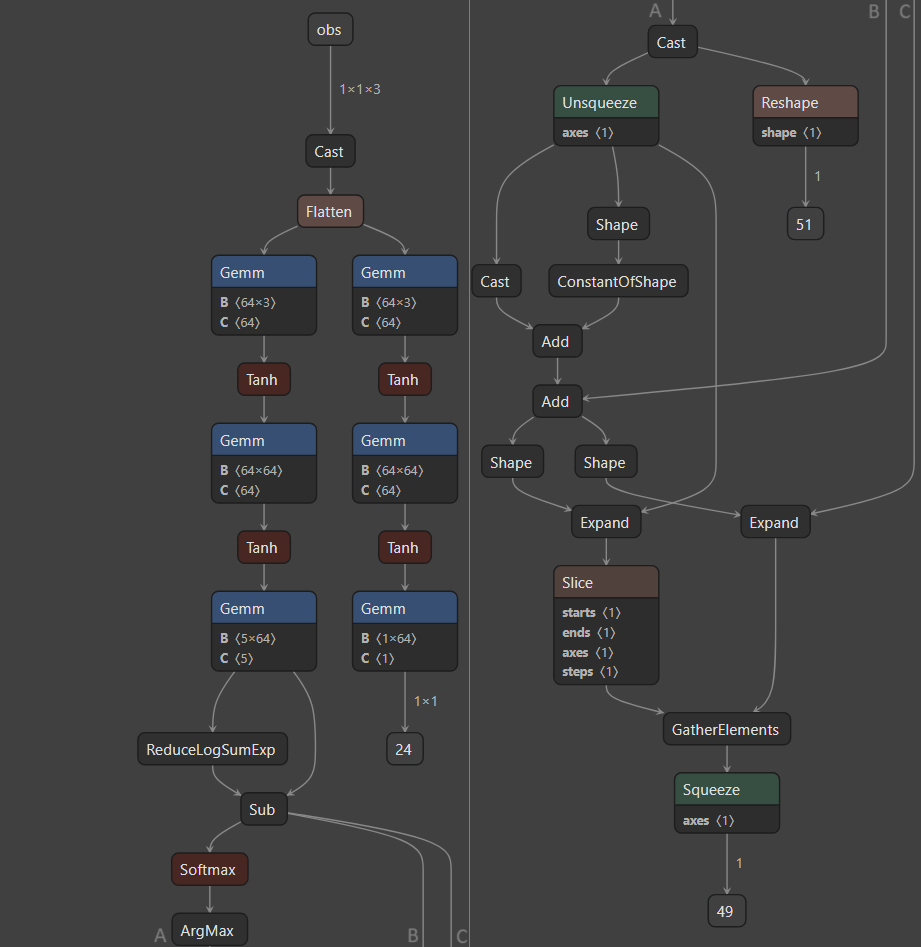
\includegraphics[scale=0.6]{3-1.png} 
\centering
\caption{Vzhled modelu z první verze agenta}
\label{obrModel1} 
\end{figure}

Pro představu lze v obrázku \ref{obrModel1} vidět exportovaný ONNX model první verze. Model reprezentuje jednoduchou neuronovou síť typu MLP se dvěma skrytými vrstvami a převážně actor–critic architekturou. Vstupní pole \uv{obs} má tvar $1 \times 1 \times 3$, které je následně převedeno uzlem \uv{Cast} a zploštěno (Flatten) na trojici hodnot představujících stavové pozorování.

Síť se dále větví do dvou částí:

\begin{enumerate}
	\item Policy head (levá větev):
	\begin{itemize}
		\item obsahuje dvě plně propojené vrstvy (\uv{Gemm} $3 \to 64$ a $64 \to 64$) s aktivační funkcí \uv{Tanh}, následované výstupní vrstvou ($64 \to 5$) pro pět diskrétních akcí. Výstup je dále zpracován pomocí \uv{ReduceLogSumExp}, normalizován funkcí \uv{Softmax} a převeden pomocí \uv{ArgMax}, který vrací index akce s nejvyšší pravděpodobností.
	\end{itemize} 
	\item Value head (pravá větev):
	\begin{itemize}
		\item má stejnou strukturu skrytých vrstev ($3 \to 64$ a $64 \to 64$ s \uv{Tanh}) a končí výstupní vrstvou ($64 \to 1$), která poskytuje skalární odhad hodnoty stavu (baseline pro algoritmus PPO).
	\end{itemize} 
\end{enumerate}

V pravé části grafu jsou také podpůrné uzly (\uv{Unsqueeze}, \uv{Shape}, \uv{Slice}, \uv{GatherElements}), které slouží k úpravě tvarů tenzorů a indexování výstupů při inferenci napříč více instancemi prostředí.

\subsection{Druhá verze agenta}


\subsection{Poslední verze agenta}


\subsection{Porovnání všech verzí}


\chapter*{Závěr} % SEM NESAHEJTE!
\addcontentsline{toc}{chapter}{Závěr} % SEM NESAHEJTE!

Hlavním cílem této diplomové práce bylo navrhnout autonomního agenta, který je schopen fungovat v~dynamickém herním prostředí s~využitím metod strojového učení a~adaptovat své chování, včetně volby výbavy, s~cílem efektivně čelit protihráči.

V~úvodních kapitolách byly představeny existující přístupy k~umělé inteligenci ve hrách a~nejčastěji používané algoritmy a~techniky. Mezi analyzovanými systémy se nacházely mimo jiné AlphaStar, OpenAI Five a~Voyager; z~metod pak zejména Proximal Policy Optimization (PPO), Deep Q-Network (DQN), Self-Play a~Population-Based Training.

Následně byly popsány technologie použité při realizaci samotné hry a~agenta, především herní engine Unreal Engine a~plugin NevarokML. Součástí této části byl rovněž návrh herní logiky a~architektury agenta.

Závěrečná část práce se zaměřila na implementaci jednotlivých herních modulů, jako jsou hráčská postava, zbraně, systém kol a~mechanismy získávání výbavy, a~především na návrh, trénování a~vyhodnocení jednotlivých verzí agenta. Výsledný agent je schopen pohybu, rotace, útoku i~změny výbavy a~jeho chování je řízeno neuronovou sítí trénovanou metodami posilovaného učení.

První verze agenta byla záměrně jednoduchá a~sloužila především k~ověření práce s~pluginem NevarokML a~celým trénovacím frameworkem. Druhá verze již obsahovala kompletní bojovou logiku, avšak vykazovala nestabilní a~místy nepřirozené chování, zejména v~oblasti udržování vzdálenosti od protivníka. Finální verze agenta tyto nedostatky ve velké míře odstranila a~nejlépe prokázala schopnost adaptivního chování v~dynamickém prostředí. Agent je schopen aktivně pronásledovat protivníka, útočit a~po jednotlivých kolech upravovat svou výbavu na základě předchozích střetů.

\newpage

Navzdory dosaženým výsledkům se ukázalo, že skutečná adaptace agenta v~reálném čase během samotného hraní je výrazně omezená. Tento stav je způsoben především omezeními pluginu NevarokML. V~jeho současné podobě je například možné provozovat pouze jednoho trenéra na jedno dynamicky vytvářené herní prostředí, zatímco u~statických trénovacích map tento problém nenastává, jelikož je možné přiřadit jednomu trenérovi více prostředí. Dále není podporována změna odměnové funkce, akčního prostoru ani vstupních pozorování v~průběhu tréninku při zachování již naučeného modelu, tedy přístup známý jako Curriculum Learning, založený na postupném zvyšování obtížnosti úlohy. Z~tohoto důvodu je nutné trénovat jeden komplexní model od počátku na plně složité úloze, což výrazně omezuje možnosti dosažení optimálního chování agenta.


%%%%%%%%%%%% SEZNAM POUŽITÝCH ZDROJŮ (LITERATURA) %%%%%%%%%%%%
\clearpage  % SEM NESAHEJTE!
\addcontentsline{toc}{chapter}{Literatura} % SEM NESAHEJTE!

\begin{thebibliography}{99}   
	% formát: ČSN ISO 690. Můžete si to vygenerovat na http://www.citacepro.com (přihlaste se přes odkaz "ČVUT"), umí to vygenerovat TeX
	% řazení: abecedně podle autora (resp. prvního slova, není-li znám autor)
	
\bibitem{AlphaGo}
GOOGLE. \textit{AlphaGo}. Online. GOOGLE. Google DeepMind. B. r. Dostupné z: \url{https://deepmind.google/technologies/alphago/}. [cit. 2025-05-10].

\bibitem{ChatGPT}
CONTRIBUTORS, Wikipedia. \textit{ChatGPT}. Online. In: Wikipedia: the free encyclopedia. San Francisco (CA): Wikimedia Foundation, 2001-, https://en.wikipedia.org/wiki/Main\_Page. Dostupné z: \url{https://en.wikipedia.org/w/index.php?title=ChatGPT&oldid=1290307244}. [cit. 2025-05-10].

\bibitem{Dota2}
CONTRIBUTORS, Wikipedia. \textit{Dota 2}. Online. In: Wikipedia: the free encyclopedia. San Francisco (CA): Wikimedia Foundation, 2001-. Dostupné z: \url{https://en.wikipedia.org/w/index.php?title=Dota\_2&oldid=1288870722}. [cit. 2025-05-10].

\bibitem{Jaderberg2017}
JADERBERG, Max; DALIBARD, Valentin a OSINDERO, Simon et al. \textit{Population Based Training of Neural Networks}. Online, arxiv. USA: Cornell University, 2017. Dostupné z: \url{https://arxiv.org/abs/1711.09846}. [cit. 2025-05-10].

\bibitem{MuJoCo}
\textit{MuJoCo}. Online. C2021. Dostupné z: \url{https://mujoco.org/}. [cit. 2025-05-10].

\bibitem{OpenAIFive}
TEAM, OpenAI Five. \textit{OpenAI Five defeats Dota 2 world champions}. Online. OpenAI. 2019. Dostupné z: \url{https://openai.com/index/openai-five-defeats-dota-2-world-champions/\#timeline}. [cit. 2025-05-10].

\bibitem{PPOOpenAI}
\textit{Proximal Policy Optimization}. Online. OpenAI. 2017. Dostupné z: \url{https://openai.com/index/openai-baselines-ppo/}. [cit. 2025-05-10].

\bibitem{Schulman2015}
SCHULMAN, John; LEVINE, Sergey; MORITZ, Philipp; JORDAN, Michael I. a ABBEEL, Pieter. \textit{Trust Region Policy Optimization}. Online, arxiv. USA: Cornell University, 2015. Dostupné z: \url{http://arxiv.org/abs/1502.05477}. [cit. 2025-05-10].

\bibitem{Schulman2017}
SCHULMAN, John; WOLSKI, Filip; DHARIWAL, Prafulla; RADFORD, Alec a KLIMOV, Oleg. \textit{Proximal Policy Optimization Algorithms}. Online, arxiv. USA: Cornell University, 2017. Dostupné z: \url{https://arxiv.org/abs/1707.06347}. [cit. 2025-05-10].

\bibitem{Schulman2018}
SCHULMAN, John; MORITZ, Philipp; LEVINE, Sergey; JORDAN, Michael a ABBEEL, Pieter. \textit{High-Dimensional Continuous Control Using Generalized Advantage Estimation}. Online, arxiv. USA: Cornell University, 2018. Dostupné z: \url{https://arxiv.org/abs/1506.02438}. [cit. 2025-05-10].

\bibitem{Vinyalsbr}
VINYALS, Oriol; BABUSCHKIN, Igor; CHUNG, Junyoung et al. \textit{AlphaStar: Mastering the real-time strategy game StarCraft II}. Online. Google DeepMind. B. r. Dostupné z: \url{https://deepmind.google/discover/blog/alphastar-mastering-the-real-time-strategy-game-starcraft-ii/}. [cit. 2025-05-10].

\bibitem{Wangbr}
WANG, Guanzhi; XIE, Yuqi a JIANG, Yunfan et al. \textit{Voyager: An Open-Ended Embodied Agent with Large Language Models}. Online. MineDojo. B. r. Dostupné z: \url{https://voyager.minedojo.org/}. [cit. 2025-05-10].

\bibitem{Watkins1992}
WATKINS, Christopher J. C. H. a DAYAN, Peter. Q-learning. Online. \textit{Machine Learning}. 1992, roč. 8, č. 11, s.~279---292. Dostupné z: \url{https://doi.org/10.1007/BF00992698}. [cit. 2025-05-10].

\bibitem{WikiDB}
CONTRIBUTORS, Wikipedia. \textit{Deep Blue (chess computer)}. Online. In: Wikipedia: the free encyclopedia. San Francisco (CA): Wikimedia Foundation, 2001-. Dostupné z: \url{https://en.wikipedia.org/w/index.php?title=Deep\_Blue\_(chess\_computer)&oldid=1288103584}. [cit. 2025-05-10].

\bibitem{WikiSC}
CONTRIBUTORS, Wikipedia. \textit{StarCraft II}. Online. In: Wikipedia: the free encyclopedia. San Francisco (CA): Wikimedia Foundation, 2001-. Dostupné z: \url{https://en.wikipedia.org/w/index.php?title=StarCraft\_II&oldid=1286300229}. [cit. 2025-05-10].

\bibitem{Zhang2024}
ZHANG, Ruize; XU, Zelai a MA, Chengdong et al. \textit{A Survey on Self-play Methods in Reinforcement Learning}. Online, arxiv. USA: Cornell University, 2024. Dostupné z: \url{https://arxiv.org/abs/2408.01072}. [cit. 2025-05-10].	
	
\end{thebibliography}

%%%%%%%%%%%% PŘÍLOHY PRÁCE %%%%%%%%%%%%
\newpage % SEM NESAHEJTE!
\addcontentsline{toc}{chapter}{Přílohy} % SEM NESAHEJTE!
\appendix % SEM NESAHEJTE!


%%%%%%%%%%%% Přílohy %%%%%%%%%%%%

\chapter{Jak zapnout program}

\begin{enumerate}
\item Nejprve si stáhněte soubor přiložený k~diplomové práci z~OneDrive, který obsahuje jak samotný projekt, tak také pluginy, jež je nutné přidat do Unreal Enginu.
\item Pokud nemáte nainstalovaný \uv{Epic Games Store}, stáhněte si jej ze stránky \texttt{https://store.epicgames.com/}. V~pravém horním rohu klikněte na tlačítko \uv{Download} a~spusťte instalátor, čímž nainstalujete \uv{Epic Games Launcher}.
\item Po spuštění aplikace si vytvořte účet (pokud jej ještě nemáte), buď přímo v \uv{Epic Games Store}, nebo prostřednictvím \uv{Epic Games Launcher}, a~přihlaste se.
\item Po přihlášení klikněte v~levém menu na položku \uv{Unreal Engine}.
\item V~horní části aplikace se zobrazí nové možnosti — vyberte záložku \uv{Library}.
\item V~sekci \uv{Engine Versions} klikněte na tlačítko \uv{+}. Objeví se nabídka výběru verze enginu. Zvolte verzi \texttt{5.2.1} a~spusťte instalaci. Umístění instalace můžete ponechat výchozí, ale zapamatujte si ho — bude potřeba později.
\item Po dokončení instalace přejděte do složky s~nainstalovaným enginem, která se bude jmenovat \texttt{UE\_5.2}. Do této složky vložte podsložku \texttt{Engine} ze složky \uv{Pluginy}, která je umístěna vedle složky projektu \uv{RoboHell}. Tímto krokem zajistíte správné nainstalování potřebných pluginů.
\item Projekt spusťte dvojklikem na soubor \uv{RoboHell.uproject} ve složce projektu. První spuštění může trvat déle, protože probíhá příprava enginu a~kompilace projektu.
\item Po načtení projektu jej zatím nespouštějte pomocí zeleného trojúhelníku! Před prvním spuštěním je třeba provést ještě několik kroků.
\item V~levém horním rohu klikněte na \uv{Edit} a~v~rozbaleném menu vyberte \uv{Editor Preferences}.
\item V~zobrazeném nastavení sjeďte v~levém panelu dolů k~sekci \uv{Plugins} a~rozklikněte \uv{NevarokML}.
\item Klikněte na tlačítko \uv{Refresh Details}. Vizuálně se nic nezmění, ale tímto krokem se plugin správně načte v~editoru.
\item Tímto by mělo být vše připraveno. Projekt by nyní měl být plně funkční. Doporučuji však přečíst také kapitolu \uv{Jak opravit problém s~projektem}, která řeší častou chybu při spouštění.
\end{enumerate}


\end{document} % SEM NESAHEJTE! Konec.
